%%%%%%%%%%%%%%%%%%%%%%%%%%%%%%%%%%%%%%%%%%%%%%%%%%%%%%%%%%%%%%%%%%%%%%%%%%%%%%%%
%
%	- Introduction to Mobile Robotics - SS 2017
%		- http://ais.informatik.uni-freiburg.de/teaching/ss17/robotics/
%
%	- Robot Mapping - WS 2016/17 - Uni-Freiburg
%		- http://ais.informatik.uni-freiburg.de/teaching/ws16/mapping/
%		- https://www.youtube.com/playlist?list=PLgnQpQtFTOGQrZ4O5QzbIHgl3b1JHimN_&feature=g-list
%	
% 	- Probabilistic Robotics
%		- http://robots.stanford.edu/probabilistic-robotics/
%
%%%%%%%%%%
\chapter{Grundlagen}


%%%%%%%%%%%%%%%%%%%%%%%%%%%%%%%%%%%%%%%%%%%%%%%%%%%%%%%%%%%%%%%%%%%%%%%%%%%%%%%%
%
% https://de.wikipedia.org/wiki/Fading_(Elektrotechnik)
%
%%%%%%%%%%
\section{Verfahren für die Entfernungsbestimmung}

Bei der \textit{Triangulation} werden die Winkel zwischen mehreren Referenzpunkten bestimmt und dann die dazu gehörige Entfernung mittels trigonometrischer Funktionen berechnet. Dieses Verfahren ist auch unter den Namen \Gls{aoa} bzw. \Gls{doa} bekannt. Um eine genau Ortsbestimmung durchzuführen müssen die Winkel sehr genau bestimmt werden. Um das zu bewerkstelligen werden im Empfänger mehrere Antennen zu einem Feld (engl. Antenna Array) zusammengefasst. Jedoch ist diese Konstruktion sehr teuer und empfindlich für Mehrwegeempfang (engl. Multipath) bzw. Signalabschattungen. \cite{gezici2005localization, liu2007survey, decawave2014rtls}

Im Gegensatz dazu werden bei der \textit{Trilateration} die Entfernungen zwischen mehreren Referenzpunkten betrachtet. Es werden dabei die Verfahren \Gls{toa} und \Gls{tdoa} unterschieden.
Bei dem \Gls{toa}-Verfahren wird zuerst die Zeitdifferenz zwischen dem Senden und Empfangen eines Funksignals berechnet. Mittels der Signallaufzeit (engl. \acrfull{tof}) und der Ausbreitungsgeschwindigkeit des Funksignals kann die Entfernung berechnet werden. Die Ortsbestimmung erfolgt dann über die Schnittpunkte von drei Kreisen (2D) bzw. vier Kugeln (3D) miteinander. Um dieses Verfahren anwenden zu können, ist es erforderlich das das Funksignal mit einem Zeitstempel des Startzeitpunktes versehen ist. Daraus folgt aber auch, das die Zeit zwischen Sender und Empfänger sehr genau synchronisiert werden müssen um den Fehler möglich klein zu halten.
Bei dem \Gls{tdoa}-Verfahren werden die Zeitdifferenz zwischen dem Empfang des Funksignals an mehreren Empfängern ausgewertet. Dies hat den großen Vorteil das nur noch die Zeit zwischen den Empfängern synchronisiert werden muss. \cite{zekavat2011handbook, decawave2014rtls}

Neben der \textit{Triangulation} und \textit{Trilateration} besteht auch die Möglichkeit auf Grund der empfangenen Signalstärke (engl. \acrfull{ss_radio}, \acrfull{rss} oder auch \acrfull{rssi}) Rückschlüsse über die Entfernung zu ziehen. Dazu muss die ursprüngliche Signalstärke und die Ausbreitungscharakteristik der elektromagnetischen Welle in der spezifischen Umgebung bekannt sein. \cite{gezici2005localization, decawave2014rtls}

In den nächsten zwei Abschnitten werden die \textit{DecaWave} Entfernungsmessverfahren vorgestellt. Diese haben den Vorteil, dass keine Synchronisierung der Zeit zwischen Sender und Empfänger notwendig ist. Weiterhin besitzen die \textit{DecaWave} \Gls{uwbt} zwei Eigenschaften die die Entfernungsmessung ideal ergänzt. Zum einen wird jede erhaltene Nachricht mit einem lokalen Zeitstempel versehen, der über eine minimale Auflösung von ungefähr \SI{15.65}{\pico\second} verfügt. Hiermit wäre eine theoretische Ortsauflösung von ungefähr \SI{5}{\milli\metre} möglich. Des Weiteren ist es möglich, den Sendezeitpunkt einer Nachricht in die Zukunft zu legen. Damit lässt sich die Zeitspanne zwischen dem Empfang und der Antwort auf eine Nachricht im Voraus berechnen. Die Zeitspanne kann dann der Antwortnachricht als Nutzlast mitgegeben werden, um beim Empfänger die Umlaufzeit zu berechnen.


%%%%%%%%%%%%%%%%%%%%%%%%%%%%%%%%%%%%%%%%%%%%%%%%%%%%%%%%%%%%%%%%%%%%%%%%%%%%%%%%
%
% 	- Wie lange dauert es bis eine Nachricht ausgetauscht worden ist?
%		- Beispiel mit einer konkreten Entfernung?
%	- Wie schnell drifted ein Quarz in einem µc?
%		- What is the ppm in the crystal oscillator?
%		- https://electronics.stackexchange.com/questions/15851/what-is-the-ppm-in-the-crystal-oscillator
%		- In the 1930s, such precise time measurements simply weren't possible; a clock of the required accuracy was difficult enough to build in fixed form, let alone portable. A crystal oscillator, for instance, drifts about 1 to 2 seconds in a month, or 1.4x10−3 seconds an hour.[1] This may sound small, but as light travels 3x108 m/s, this represents a drift of 400 m per hour. Only a few hours of flight time would render such a system unusable, a situation that remained in force until the introduction of commercial atomic clocks in the 1960s.
%	- Clock accuracy in ppm
%	- http://www.best-microcontroller-projects.com/ppm.html
%
%%%%%%%%%%
\subsection{Single-sided Two-way Ranging}

Das einfachste Verfahren, um aus der Umlaufzeit die Entfernung abzuschätzen, ist das \Gls{sstwr}-Verfahren. Dabei sendet der \Gls{tag} eine Nachricht an den \Gls{anchor} und wartet ab, bis eine entsprechende Antwortnachricht eintrifft. Beide Module erhalten einen Zeitstempel für den Versand und Empfang von Nachrichten. Aus diesen kann dann die Antwort- ($T_{reply}$) und Umlaufzeit ($T_{round}$) berechnet werden, siehe \autoref{fig:single_sided_two_way_ranging}. \cite{decawave2015twr, decawave2016dw1kusermanual}

%\begin{figure}[ht]
\begin{figure}
	\centering
	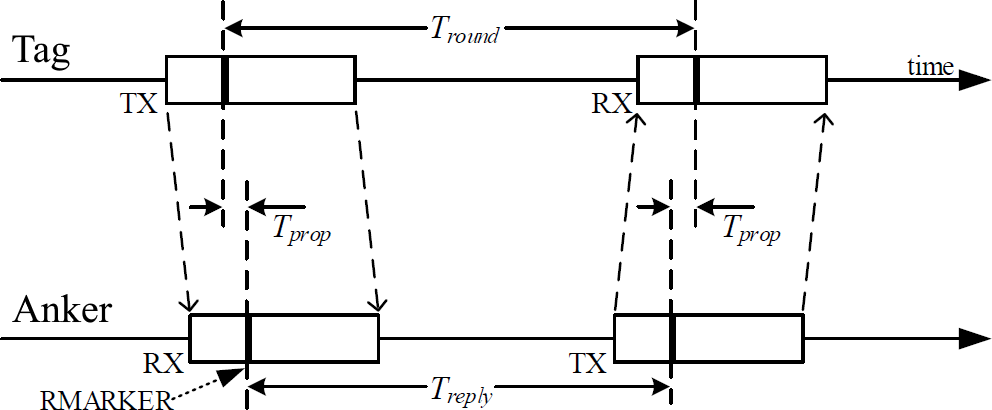
\includegraphics[width=0.75\linewidth]{single_sided_two_way_ranging}
	\captionwithcite{Ablauf des \acrlong{sstwr}.}{\cite{decawave2016dw1kusermanual}}
	\label{fig:single_sided_two_way_ranging}
\end{figure}

Die ungefähre \Gls{tof}-Zeitspanne ergibt sich aus der folgenden Gleichung:

\begin{equation}
T_{prop}=\frac{1}{2}\left(T_{round}-T_{reply}\right)
\end{equation}

Damit der \Gls{tag} die \Gls{tof}-Zeitspanne berechnen kann, benötigt er die $T_{reply}$-Zeitspanne. Zu diesem Problem gibt es mehrere Lösungen. Die einfachste Lösung ist eine feste Antwortzeit die jedem Modul bekannt ist. Alternativ kann der \Gls{anchor} in der Antwortnachricht seine individuelle Antwortzeit übermitteln. Oder der \Gls{tag} übermittelt dem \Gls{anchor} mit der initialen Nachricht wie lange der \Gls{anchor} warten muss bis er die Antwortnachricht verschickt. Hierbei muss die Zeitspanne groß genug gewählt sein, um den \Gls{anchor} die Möglichkeit zur Antwort zu lassen. Je nach Anforderung wird eine der vorherigen Methoden verwendet.

Der Nachteil bei diesem Verfahren besteht in dem Fehler der von der Antwortzeit abhängt. Bei Module verwenden zur Berechnung von $T_{round}$ und $T_{reply}$ ihre lokalen Zeitgeber. Beide Zeitgeber haben einen Offsetfehler $e_{A}$ und $e_{B}$ der von der Nennfrequenz abweicht. Die daraus abgeleitete \Gls{tof}-Zeitschätzung hat damit einen Fehler der mit der Antwortzeit wächst:

\begin{equation}
error\approx\frac{1}{2}\left(e_B-e_A\right)\times T_{reply}
\end{equation}


%%%%%%%%%%%%%%%%%%%%%%%%%%%%%%%%%%%%%%%%%%%%%%%%%%%%%%%%%%%%%%%%%%%%%%%%%%%%%%%%
%
% \cite{decawave2016dw1kusermanual}
%	- Where the clock in device A runs at ka times the desired frequency and the clock in device B runs at kb times the desired frequency and both ka & kb are close to 1.
%	- To give some idea of the size of this error, if devices A and B have clocks where each are 20 ppm away (the worst case specification) from the nominal clock in directions which make their combined error additive and equal to 40 ppm, then ka and kb might both be 0.99998 or 1.00002.
%	- Even with a relatively large UWB operating range of say 100 m, the TOF is just 333 ns, so the error is 20 × 10-6 × 333 × 10-9 seconds, which is 6.7 × 10-12 seconds or 6.7 picoseconds which is approximately 2.2 mm.
%
%%%%%%%%%%
\subsection{Double-sided Two-way Ranging}
\label{subsec:double_sided_two_way_ranging}

Das \Gls{dstwr}-Verfahren stellt eine Verbesserung gegenüber dem \Gls{sstwr}-Verfahren dar. Hierbei werden nun drei Nachrichten verwendet um jeweils die Umlaufzeiten zwischen \Gls{tag} und \Gls{anchor}, und \Gls{anchor} und \Gls{tag} zu berechnen, siehe \autoref{fig:double_sided_two_way_ranging}. Wenn die Umlaufzeit beim \Gls{tag} berechnet werden soll, müssen die Zeitspannen $T_{reply1}$ und $T_{round2}$ zum \Gls{tag} übermittelt werden. Für die letzte Zeitspanne erfolgt das mit einer vierten Nachricht die in dem Schaubild nicht abgebildet ist. \cite{decawave2015twr, decawave2016dw1kusermanual}

%\begin{figure}[ht]
\begin{figure}
	\centering
%	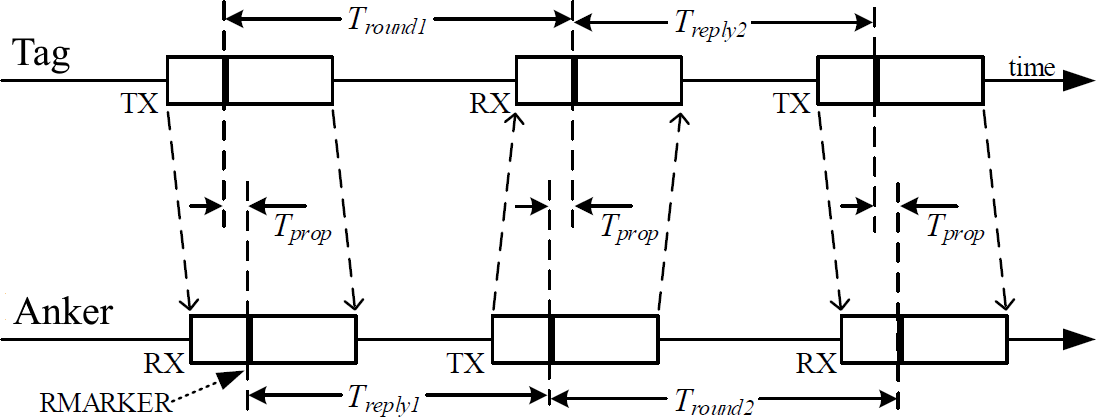
\includegraphics[width=0.7\linewidth]{double_sided_two_way_ranging}
	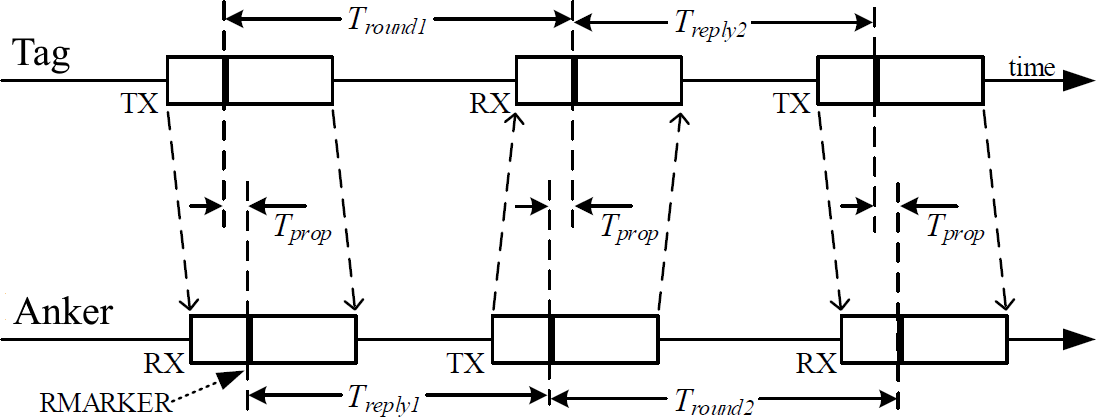
\includegraphics[width=0.8\linewidth]{double_sided_two_way_ranging}
	\captionwithcite{Ablauf des \acrlong{dstwr}.}{\cite{decawave2016dw1kusermanual}} 
	\label{fig:double_sided_two_way_ranging}
\end{figure}

Die ungefähre \Gls{tof}-Zeitspanne ergibt sich aus der folgenden Gleichung:

\begin{equation}
T_{prop} = \frac{\left(T_{round1}\times T_{round2}-T_{reply1}\times T_{reply2}\right)}{\left(T_{round1}+T_{round2}+T_{reply1}+T_{reply2}\right)}
\end{equation}

Der Fehler bei diesem Verfahren ergibt sich aus der folgenden Gleichung:

\begin{equation}
error=T_{prop}\times\left(1-\frac{k_a+k_b}{2}\right)
\end{equation}

Die Variablen $k_a$ und $k_b$ entsprechen hierbei den Offsetfehler der Zeitgeber von der Nennfrequenz und liegen beide sehr nahe bei eins.

Mit diesem Verfahren ist es auch möglich, gleichzeitig die Entfernungen zu mehr als einem \Gls{anchor} zu bestimmen, siehe \autoref{fig:double_sided_two_way_ranging_with_three_anchor}. Hierbei weist der \Gls{tag} in der initialen Nachricht jedem \Gls{anchor} eine individuelle Antwortzeit zu. Danach wartet er bist alle Antwortnachrichten angekommen sind um im der letzten Nachricht, dann jedem \Gls{anchor} seine Umlauf- und Antwortzeiten zu übermitteln. Jeder \Gls{anchor} kann nun individuell die \Gls{tof}-Zeitspanne für sich berechnen und dann dem \Gls{tag} übermitteln. Diese letzte Nachricht ist auf der \autoref{fig:double_sided_two_way_ranging_with_three_anchor} nicht aufgeführt.

%\begin{figure}[ht]
\begin{figure}
	\centering
	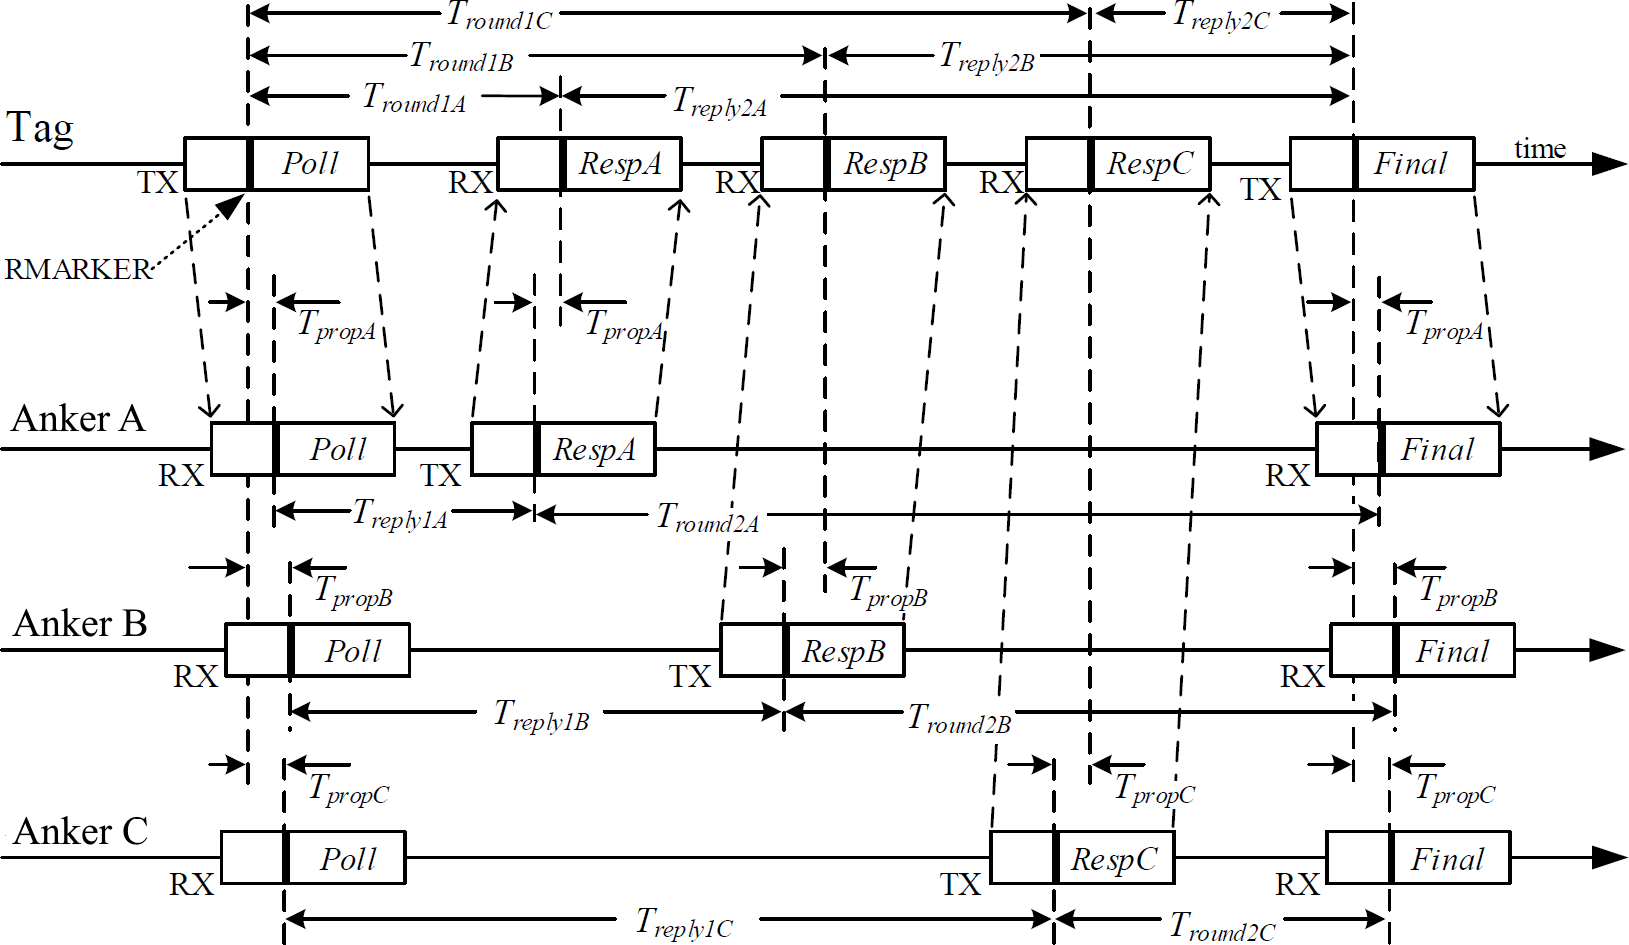
\includegraphics[width=\linewidth]{double_sided_two_way_ranging_with_three_anchor}
	\captionwithcite{Ablauf des \acrlong{dstwr} mit einem \Gls{tag} und drei \Gls{anchor}.}{\cite{decawave2016dw1kusermanual}}
	\label{fig:double_sided_two_way_ranging_with_three_anchor}
\end{figure}

In der \autoref{fig:double_sided_two_way_ranging_with_three_anchor} wurde in der initialen Nachricht jedem \Gls{anchor} eine individuelle Antwortzeit zugeordnet. Woher wusste der\Gls{tag} welche \Gls{anchor} vorhanden sind? Die Kommunikation zwischen \Gls{tag} und \Gls{anchor} kann in zwei Phasen unterteilt werden, siehe \autoref{fig:discovery_and_ranging_phase}. In der \textit{Discovery} Phase schickt der \Gls{tag} periodisch \textit{Blink} Nachrichten mit seiner Identifikationsnummer an alle Module in der Umgebung. Empfängt ein \Gls{anchor} diese Nachricht, nimmt er den \Gls{tag} in seiner Liste auf und übermittelt dem \Gls{tag} eine \textit{Ranging Init} Nachricht mit seiner Identifikationsnummer. Das \Gls{tag} seinerseits nimmt den \Gls{anchor} in seiner Liste auf und weiß nun auch welche \Gls{anchor} er in der nächsten Entfernungsmessung berücksichtigen muss. Die \textit{Ranging} Phase entspricht hierbei der bereits zuvor besprochenen Entfernungsmessung.

%\begin{figure}[ht]
\begin{figure}
	\centering
%	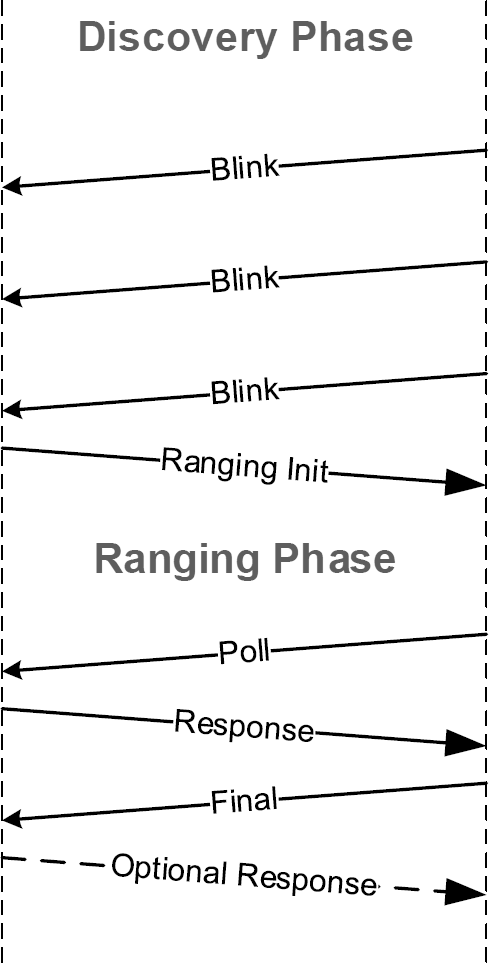
\includegraphics[width=0.4\linewidth]{discovery_and_ranging_phase2}
	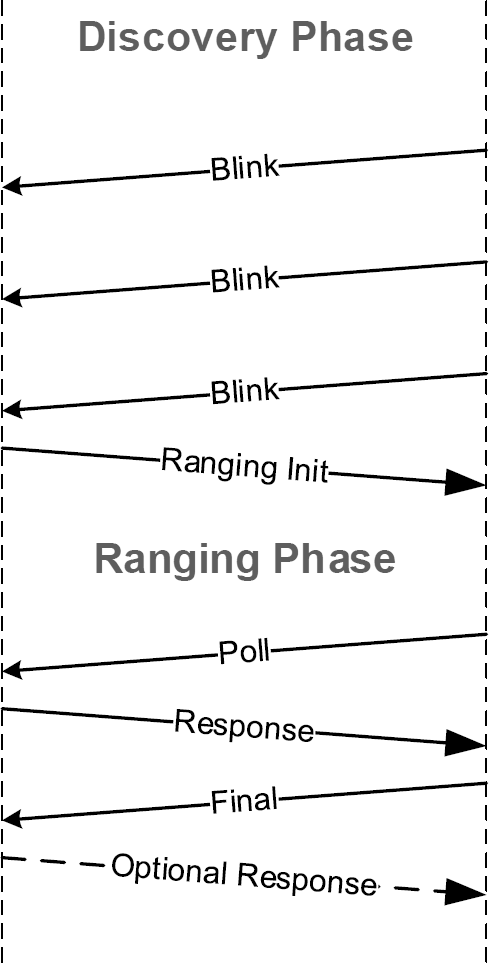
\includegraphics[width=0.3\linewidth]{discovery_and_ranging_phase2}
	\captionwithcite{Ablauf der \textit{Discovery} und \textit{Range Phase} zwischen einem \Gls{tag} und mehreren \Gls{anchor}n.}{\cite{decawave2016dw1kusermanual}}
	\label{fig:discovery_and_ranging_phase}
\end{figure}


%%%%%%%%%%%%%%%%%%%%%%%%%%%%%%%%%%%%%%%%%%%%%%%%%%%%%%%%%%%%%%%%%%%%%%%%%%%%%%%%
%
%
%
%%%%%%%%%%
\section{Geometrie}


%%%%%%%%%%%%%%%%%%%%%%%%%%%%%%%%%%%%%%%%%%%%%%%%%%%%%%%%%%%%%%%%%%%%%%%%%%%%%%%%
%
%
%
%%%%%%%%%%
\subsection{Gleichseitiges Dreieck}

Ein gleichseitiges Dreieck zeichnet sich dadurch aus, dass alle drei Seiten gleich lang sind und jeder Innenwinkel einen Wert von \SI{60}{\degree} besitzt, siehe \autoref{fig:wikipedia_gleichseitiges_dreieck}. Ist der Umkreisradius $r_u$ eines gleichseitigen Dreiecks bekannt, so kann mit der \autoref{eq:dreieck_seitenlaenge_aus_umkreis} auch die Seitenlänge $a$ berechnet werden.

\begin{equation}
a = \frac{3}{\sqrt{3}} r_u \label{eq:dreieck_seitenlaenge_aus_umkreis}
\end{equation}


%%%%%%%%%%%%%%%%%%%%%%%%%%%%%%%%%%%%%%%%%%%%%%%%%%%%%%%%%%%%%%%%%%%%%%%%%%%%%%%%
%
%
%
%%%%%%%%%%
\subsection{Regelmäßiges Fünfeck}

Das regelmäßige Fünfeck zeichnet sich dadurch aus, das alle fünf äußeren Seiten gleich lang sind und jeder Innenwinkel einen von Wert von \SI{108}{\degree} besitzt, siehe \autoref{fig:wikipedia_regelmaessiges_fuenfeck}. Aus der Länge einer äußeren Seite $a$ lässt sich zum einen der Umkreisradius $r_u$, siehe \autoref{eq:fuenfeck_umkreisradius}, und die Diagonale $d$ zwischen zwei Spitzen, siehe \autoref{eq:fuenfeck_diagonale}, berechnen.

\begin{equation}
r_u = \frac{a}{10} \sqrt{50 + 10 \sqrt{5}} \label{eq:fuenfeck_umkreisradius}
\end{equation}

\begin{equation}
d = \frac{a}{2} \left(1 + \sqrt{5} \right) \label{eq:fuenfeck_diagonale}
\end{equation}


%%%%%%%%%%%%%%%%%%%%%%%%%%%%%%%%%%%%%%%%%%%%%%%%%%%%%%%%%%%%%%%%%%%%%%%%%%%%%%%%
%
%	- Bayesian statistics
%		- https://en.wikipedia.org/wiki/Bayesian_statistics
%	- Law of total probability
%		- https://en.wikipedia.org/wiki/Law_of_total_probability
%	- Rule of Total Probability and Bayes' Rule
%		- https://www.youtube.com/watch?v=VvThd5zRQC4
%		- https://www.youtube.com/watch?v=8SCmdX68pIk
%	- Zufallsvariable, Massenfunktion, Dichtefunktion und Verteilungsfunktion
%		- https://www.youtube.com/watch?v=DoHTsDrzAQk
%	- A modern introduction to probability and statistics.pdf
%
%%%%%%%%%%
\section{Wahrscheinlichkeitstheorie}

Ob sich ein Roboter an einer ganz bestimmten Position befindet, lässt sich in der Praxis nicht genau bestimmen. Auch durch das genauere Vermessen der Position bleibt eine gewisse Unsicherheit. Um diese Unsicherheit abzubilden, wird in der Robotik die Wahrscheinlichkeitstheorie angewendet. Zum Einsatz kommen hierbei kontinuierliche Zufallsvariablen und die mit ihnen verbundene \Gls{wdf}. In der Regel wird eine Gaußsche Normalverteilung eingesetzt, die sich über den Mittelwert $\mu$ und Varianz $\sigma^2$ beschreiben lässt, siehe \autoref{eq:normal_distribution}. Häufig wird die Normalverteilung auch über $\operatorname{\mathcal{N}}{(x; \mu, \sigma^2)}$ abgekürzt.

\begin{equation}
p(x) = \left( 2 \pi \sigma^2 \right)^{-\frac12}  \exp{ \left\{ -\frac12 \frac{(x - \mu)^2}{\sigma^2} \right\} } \label{eq:normal_distribution}
\end{equation}

Da es sich bei der Position nicht um einen skalaren Wert handelt, muss eine mehrdimensionale Normalverteilung eingesetzt werden, siehe \autoref{eq:multivariate_normal_distribution}. Diese wird über einen Vektor der Mittelwerte $\mu$ und eine symmetische Kovarianzmatrix $\Sigma$ beschrieben.

\begin{equation}
p(x) = \operatorname{det}{\left( 2 \pi \Sigma \right)}^{-\frac12}  \exp{ \left\{ -\frac12 (x - \mu)^T \Sigma^{-1} (x - \mu) \right\} } \label{eq:multivariate_normal_distribution}
\end{equation}

Die Multivariate Verteilung zweier Zufallsvariablen beschreibt die Wahrscheinlichkeit, mit welcher das Ereignis $x$ sowie das Ereignis $y$ auftritt. Sollten beide Zufallsvariablen unabhängig von einander sein, so lassen sich ihre Wahrscheinlichkeiten multiplizieren, siehe \autoref{eq:independent_joint_distribution}.

\begin{equation}
p(x, y) = p(x) \, p(y) \label{eq:independent_joint_distribution}
\end{equation}

Von der bedingten Wahrscheinlichkeit spricht man dann, wenn eine Zufallsvariable, Wissen über eine anderen Zufallsvariable besitzt, siehe \autoref{eq:conditional_probability}.

\begin{equation}
p(x \mid y) = \frac{p(x, y)}{p(y)} \label{eq:conditional_probability}
\end{equation}

Die bedingte Wahrscheinlichkeit von zwei Zufallsvariablen die unabhängig von einander sind, reduzieren sich zu der Wahrscheinlichkeit einer Zufallsvariable, siehe \autoref{eq:independent_joint_distribution} und \autoref{eq:independent_conditional_probability}.

\begin{equation}
p(x \mid y) = \frac{p(x) \, p(y)}{p(y)} = p(x) \label{eq:independent_conditional_probability}
\end{equation}

Der Satz von Bayes sagt aus, das ein Verhältnis zwischen der bedingten Wahrscheinlichkeit $p(x \mid y)$ und der umgekehrten Form $p(y \mid x)$ besteht, siehe \autoref{eq:bayes_rule}.

\begin{equation}
p(x \mid y) = \frac{p(y \mid x) \, p(x)}{p(y)} \label{eq:bayes_rule}
\end{equation}

Der Nenner $p(y)$ hängt nicht von $x$ ab, ist daher für jedes Ereignis konstant und wird als Konstante $\eta$ vor die Gleichung gesetzt, siehe \autoref{eq:bayes_rule_with_normalizer}.

\begin{equation}
p(x \mid y) = \eta \, p(y \mid x) \, p(x) \label{eq:bayes_rule_with_normalizer}
\end{equation}


%%%%%%%%%%%%%%%%%%%%%%%%%%%%%%%%%%%%%%%%%%%%%%%%%%%%%%%%%%%%%%%%%%%%%%%%%%%%%%%%
%
%
%
%%%%%%%%%%
\section{Zustandsschätzer}

Ein Roboter der sich in seiner Umwelt zurechtfinden soll, muss diese modellieren. Das Ergebnis der Modellierung bezeichnet man als Zustand. Ein Zustand beschreibt dabei alle Aspekte des Roboters und seiner Umwelt die einen Einfluss auf die Zukunft haben können. Ein Zustand kann dabei aus statischen sowie dynamischen Komponenten bestehen. Aus dem letzteren ergibt sich zwangsweise, dass ein Zustand sich auch über die Zeit verändern kann. Ein Zustand kann z.B. die Pose des Roboters sein, die Positionen von stationären Landmarken oder aber auch der Ladezustand der Energieversorgung. Beschrieben wird er Zustand mit dem Symbol $x$.

Die meisten Roboter verfügen über Sensoren um Änderungen an Ihrer Umwelt wahrzunehmen. Diese Wahrnehmungen werden dabei mit dem Symbol $z$ beschrieben. Zusätzlich kann der Roboter aktiv Änderungen an seiner Umwelt vornehmen, in dem er Steuerbefehle and die Aktorik sendet und sich somit durch seine Umwelt bewegt. Steuerbefehle werden mit dem Symbol $u$ beschrieben.

Um Auszudrücken, dass die Information des Zustandes, der Wahrnehmung und der Steuerbefehle, zu einem bestimmen Zeitpunkt gehören wird der Index $x_t$ verwendet. Eine Zeitspanne wird über den Index $x_{1:t}$ ausgedrückt. Im mathematischen Sinne werden alle drei Größe als Spaltenvektoren beschrieben, die nicht über die gleiche Dimension verfügen müssen. Zum Beispiel könnte der Zustand aus den X-/Y-Position und der Orientierung $\theta$ zusammengesetzt sein, während die Wahrnehmung aus vielen hunderten Entfernungsmessungen bestehen.

Der Zustand der Umwelt kann nicht direkt gemessen werden, stattdessen muss dieser aus den Daten der Wahrnehmung und der Steuerbefehle geschlussfolgert werden. Das interne Wissen des Roboters über den Zustand seiner Umwelt wird dabei als Belief $bel(x_t)$ bezeichnet. Der Belief wird dabei durch eine bedingte Wahrscheinlichkeitsverteilung repräsentiert. Jeder Zustandshypothese ordnet der Belief dabei eine Wahrscheinlichkeit für ihre Gültigkeit zu.


%%%%%%%%%%%%%%%%%%%%%%%%%%%%%%%%%%%%%%%%%%%%%%%%%%%%%%%%%%%%%%%%%%%%%%%%%%%%%%%%
%
%	- A Short Introduction to the Bayes Filter and Related Models
%		- http://ais.informatik.uni-freiburg.de/teaching/ws12/mapping/pdf/slam02-bayes-filter-short.pdf
%	- Bayes Filter
%		- https://www.tu-chemnitz.de/informatik/KI/edu/robotik/ws2012/robotik_6_2.pdf
%
%%%%%%%%%%
\subsection{Bayes Filter}

Bei dem Bayes Filter Algorithmus handelt es sich um einen sehr abstrakte Beschreibung eines rekursiven Zustandsschätzer, siehe \autoref{fig:algorithm_bayes_filter}. Das heißt, aufbauend  auf der aktuellen Zustandsschätzung wird mit dem eintreffen neuer Wahrnehmungs- oder Steuerbefehl-Daten eine neue Zustandschätzung generiert. Abhängig vom Vorwissen des initialen Zustandes $bel(x_0)$ liefert diese entweder eine punktförmige Verteilung durch den initialen Zustand zurück oder eine stetige Gleichverteilung über den kompletten Zustandsraum. 

\begin{figure}
	\centering
	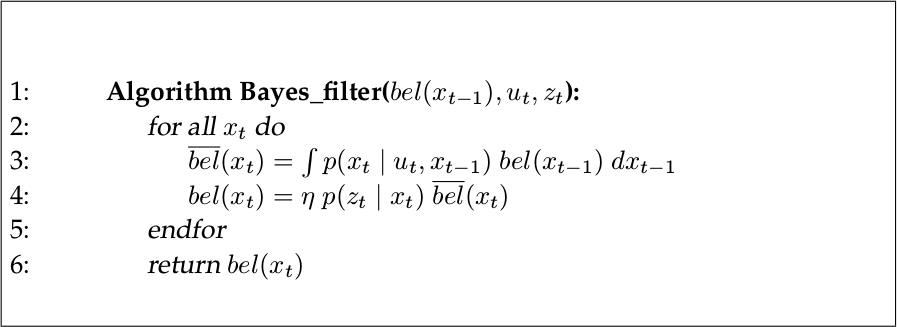
\includegraphics[width=0.7\linewidth]{algorithm_bayes_filter}
	\captionwithcite{Bayes Filter Algorithmus}{\cite{thrun2005probabilistic}}
	\label{fig:algorithm_bayes_filter}
\end{figure}

Der Bayes Filter geht dabei in zwei Schritt vor. Im ersten Schritt wird eine Prognose (engl. prediction) für den neuen Zustand erstellt, siehe Zeile 3. Der neue Zustand wird dabei aus dem vorherigen Zustand und dem aktuellen Steuerbefehl gebildet, siehe $p(x_t \mid, u_t, x_{t-1})$. Die daraus resultierende Verteilung wird mit der vorherige Belief Verteilung $bel(x_{t-1})$ multipliziert und ergibt die Prognose $\overline{bel}(x_t)$ für den neuen Zustand. Im zweite Schritt wird die erstellt Prognose mit der aktuellen Wahrnehmung korrigiert (engl. correction), siehe Zeile 4. Hierbei ist zu beachten, das für jede Zustandshypothese $x_t$ die erstelle Prognose $\overline{bel}(x_t)$ mit der Wahrscheinlichkeit multiplilziert wird, das die Wahrnehmung zu der Zustandprognose zutrifft $p(z_t \mid x_t)$.


%%%%%%%%%%%%%%%%%%%%%%%%%%%%%%%%%%%%%%%%%%%%%%%%%%%%%%%%%%%%%%%%%%%%%%%%%%%%%%%%
%
%	- Kalman fitering
%		- Multivariate Gaussian distribution (Mehrdimensionale Normalverteilung)
%		- \url{https://de.wikipedia.org/wiki/Mehrdimensionale_Normalverteilung}
%		- Kompakte Beschreibung der Normalverteilung über den Erwartungswert $\mu$ und die Kovarianzmatrix $\Sigma$ ($\mu$ und $\sigma^2$)
%		- \url{https://matheguru.com/stochastik/normalverteilung.html}
%	- Special Topics - The Kalman Filter (1 of 55) What is a Kalman Filter?
%		- https://www.youtube.com/watch?v=CaCcOwJPytQ
%	- Introduction_to_Kalman_Filtering.pdf
%
%%%%%%%%%%
\subsection{Kalman Filter}

Die Familie der Gauß Filter, zu denen auch der Kalman Filter gehört, ist eine der frühsten konkreten Implementierungen des Bayes Filters. Die Idee hinter jedem Gauß Filter liegt dabei, das der Belief durch eine mehrdimensionale Normalverteilung repräsentiert wird, die eindeutig durch die ersten beiden Momente Mittelwert $\mu$ und Kovarianz $\Sigma$ beschrieben wird. Der große Vorteil einer normalverteilten Zufallsvariable ist, dass das Ergebnis einer Lineartransformation mit einer anderen normalverteilten Zufallsvariable wieder zu einer normalverteilten Zufallsvariable führt. Zu den Nachteilen zählt, dass der Gauß Filter nur im kontinuierlichen Zustandsraum angewendet werden kann und durch die unimodale Verteilung nur für die Positionsverfolgung (engl. Position Tracking Problem) in Frage kommt.

Genauso wie der Bayes Filter geht auch der Kalman Filter in zwei Schritten vor, siehe \autoref{fig:algorithm_kalman_filter}. Im ersten Schritt wird aus dem vorherigen Zustand $\mu_{t-1}$ und $\Sigma_{t-1}$ und den aktuellen Steuerbefehlen $u_t$ die Prognose für den neuen Zustand berechnet, siehe Zeile 2--3. Über die Matrix $A_t$ wird festgelegt, wie sich der Zustand von $t-1$ nach $t$ entwickelt, ohne die Einwirkungen der Steuerbefehle oder von Rauschen. Die Matrix $B_t$ beschreibt wie die Steuerbefehle die Zustandsänderung von $t-1$ nach $t$ beeinflussen. Im zweiten Schritt wird zuerst der Kalman Gain $K_t$ berechnet, siehe Zeile 4. Bei dem Kalman Gain handelt es sich um ein Gewicht, das entscheidet wie stark die Prognose mit der Wahrnehmung korrigiert wird, siehe Zeile 5--6. Bei der Matrix $C_t$ wird definiert wir die Wahrnehmungen auf den Zustand abgebildet werden. Die beiden Matrizen $R_t$ und $Q_t$ bilden dabei das unabhängige und zufällig normalverteilte Rauschen ab.

\begin{figure}
	\centering
	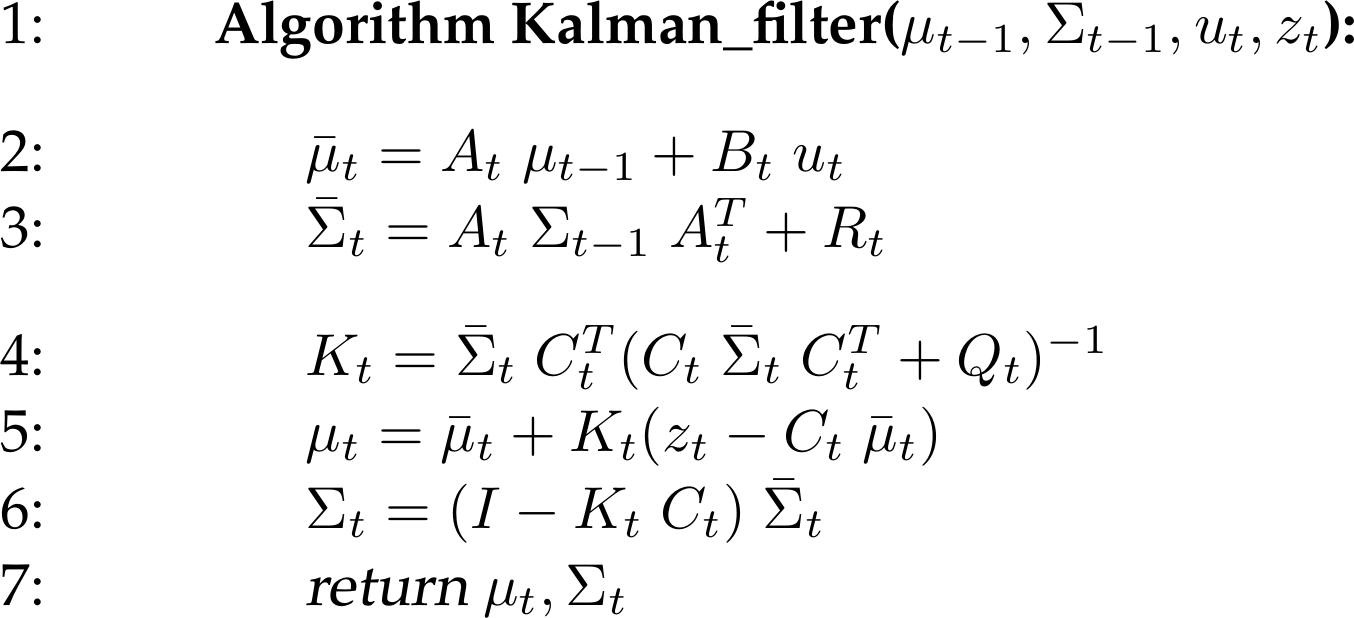
\includegraphics[width=0.7\linewidth]{algorithm_kalman_filter}
	\captionwithcite{Kalman Filter Algorithmus}{\cite{thrun2005probabilistic}}
	\label{fig:algorithm_kalman_filter}
\end{figure}


%%%%%%%%%%%%%%%%%%%%%%%%%%%%%%%%%%%%%%%%%%%%%%%%%%%%%%%%%%%%%%%%%%%%%%%%%%%%%%%%
%
%
%
%%%%%%%%%%
\subsection{Extended Kalman Filter}

Der Kalman Filter geht von der Annahme aus, dass die Zustandsänderung und die Wahrnehmungen durch eine lineare Funktion beschrieben werden können. Diese Annahme ist entscheidend für das ordnungsgemäße Funktionieren des Kalman Filters. In der \autoref{fig:random_variable_linear_transformation} ist im rechten unteren Bereich die Zufallsvariable $x$ mit ihrer Normalverteilung dargestellt. Wird diese über eine lineare Funktion $y=ax+b$ auf die Zufallsvariable $y$ abgebildet. Es ist klar zu erkennen, dass die Normalverteilung für die Zufallsvariable $y$ erhalten bleibt.

Das Hauptproblem bei der linearen Annahme ist, dass viele Zustandsänderung und Wahrnehmungen nicht mit einer linearen Funktion beschrieben werden können, z.B. rotatorische Zustandsänderungen. Die \autoref{fig:random_variable_non_linear_transformation} verdeutlich, was mit der Normalverteilung einer Zufallsvariable $x$ passiert, wenn diese durch eine nicht lineare Funktion $g(x)$ abgebildet wird. Von der Normalverteilung der Zufallsvariable $y$ bleibt nicht mehr viel übrig.

Der \Gls{ekf} löst das Problem in dem eine Linearisierung der nicht linearen Funktion vorgenommen wird, siehe \autoref{fig:random_variable_taylor_linearization}. Hierzu wird eine Taylorreihe des ersten Grades gebildet. Der Funktionswert der Mittelwertes $g(\mu)$ dient dabei als Entwicklungsstelle. Durch die Linearisierung wird die Normalverteilung der Zufallsvariable $x$ wieder ordnungsgemäß auf die Zufallsvariable $y$ abgebildet. Da es sich bei der Linearisierung nicht um die Originalfunktion handelt entsteht ein Linearisierungsfehler der am Unterschied zwischen der durchgezogen und gestrichelten Kurve zu erkennen ist.

\begin{figure}
	\centering
	\begin{subfigure}{0.49\linewidth}
		\centering
		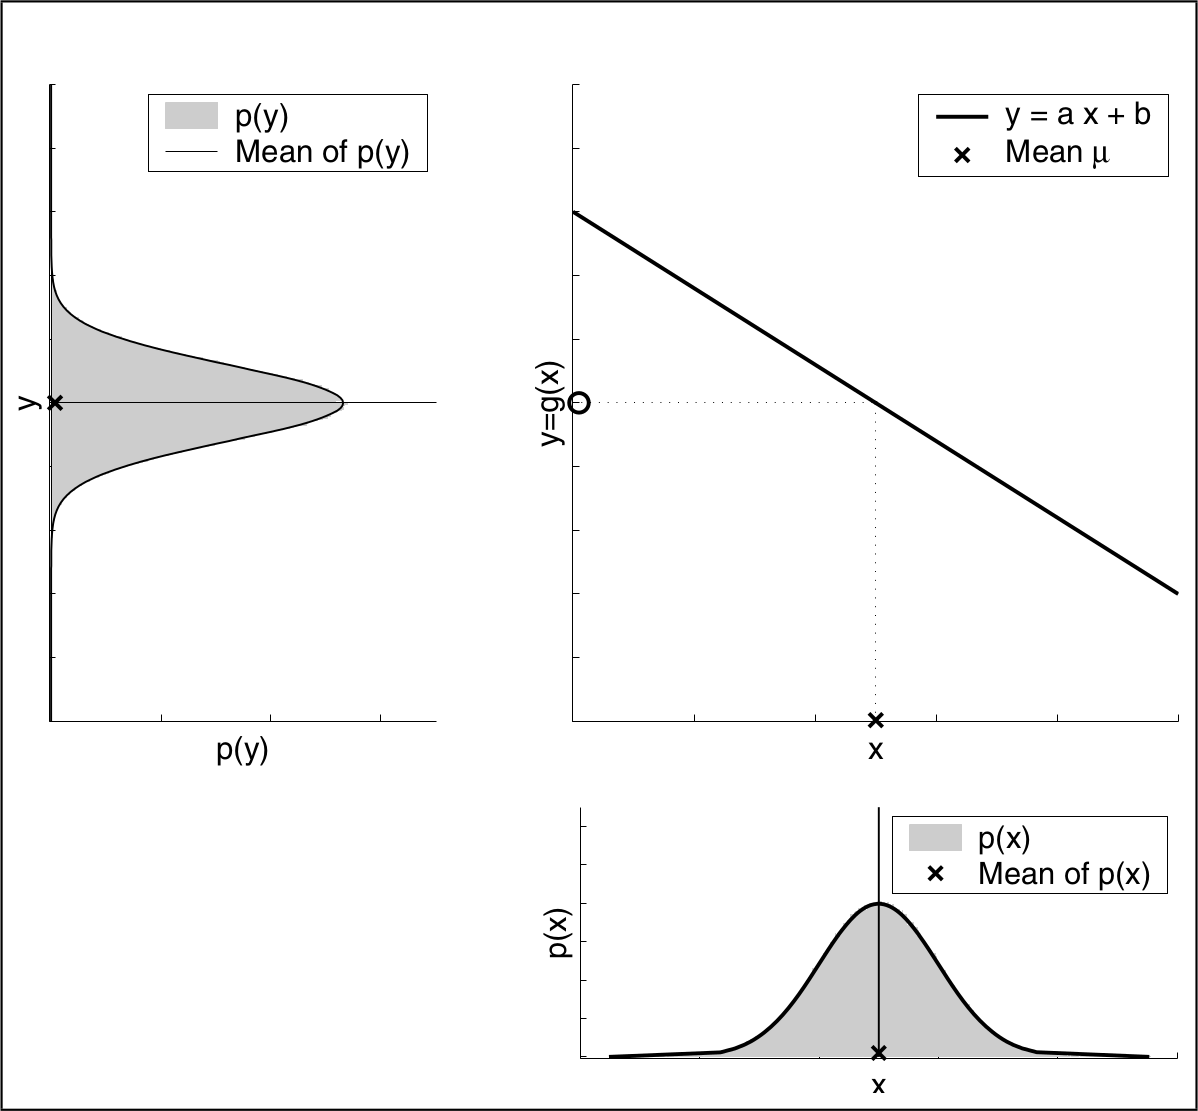
\includegraphics[width=\linewidth]{random_variable_linear_transformation}
		\caption{}
		\label{fig:random_variable_linear_transformation}
	\end{subfigure}
	\hfill
	\begin{subfigure}{0.49\linewidth}
		\centering
		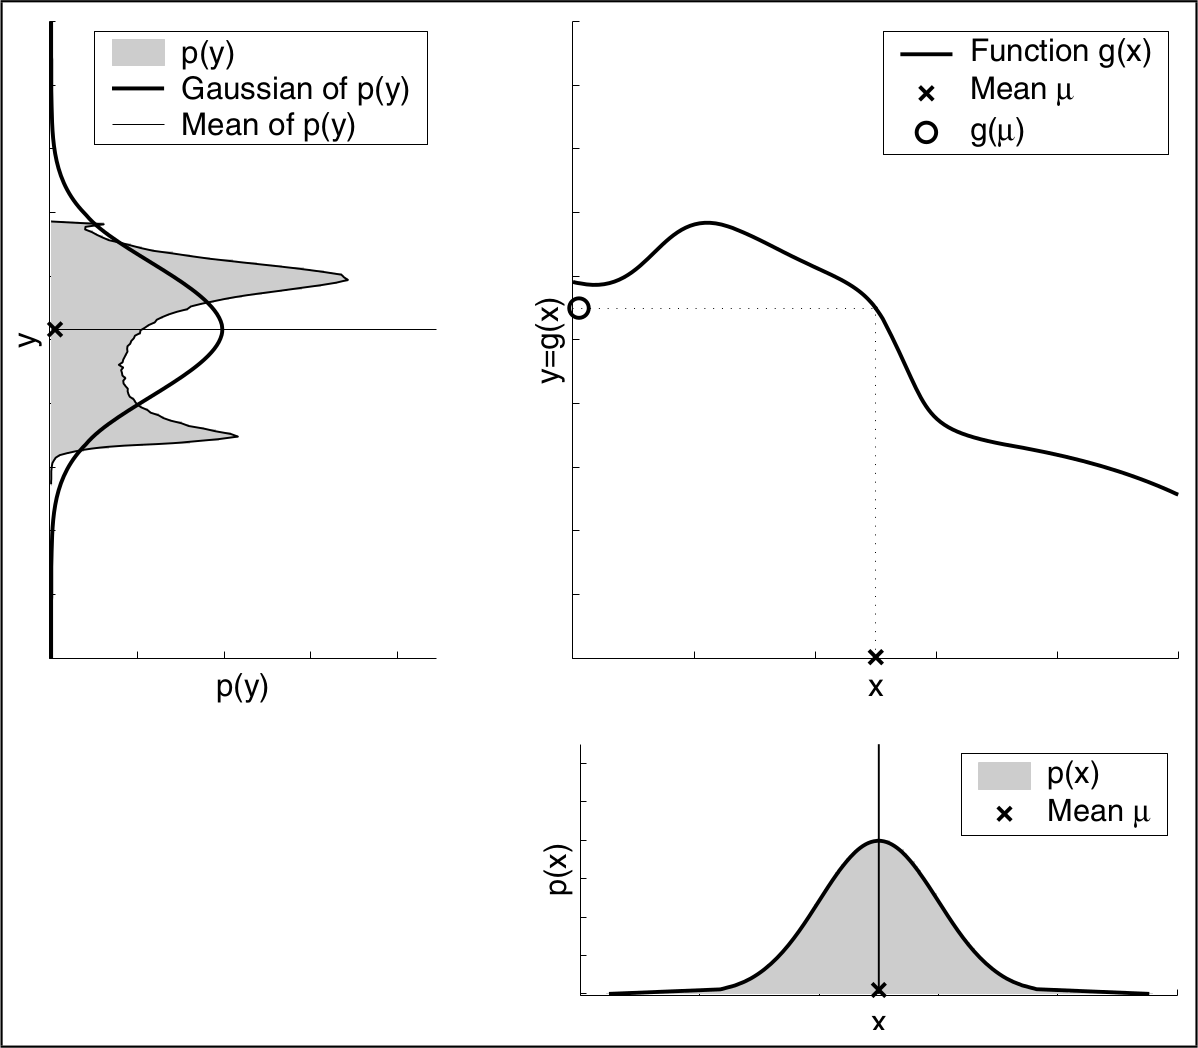
\includegraphics[width=\linewidth]{random_variable_non_linear_transformation}
		\caption{}
		\label{fig:random_variable_non_linear_transformation}
	\end{subfigure}
	\par
	\bigskip
	\begin{subfigure}{0.49\linewidth}
		\centering
		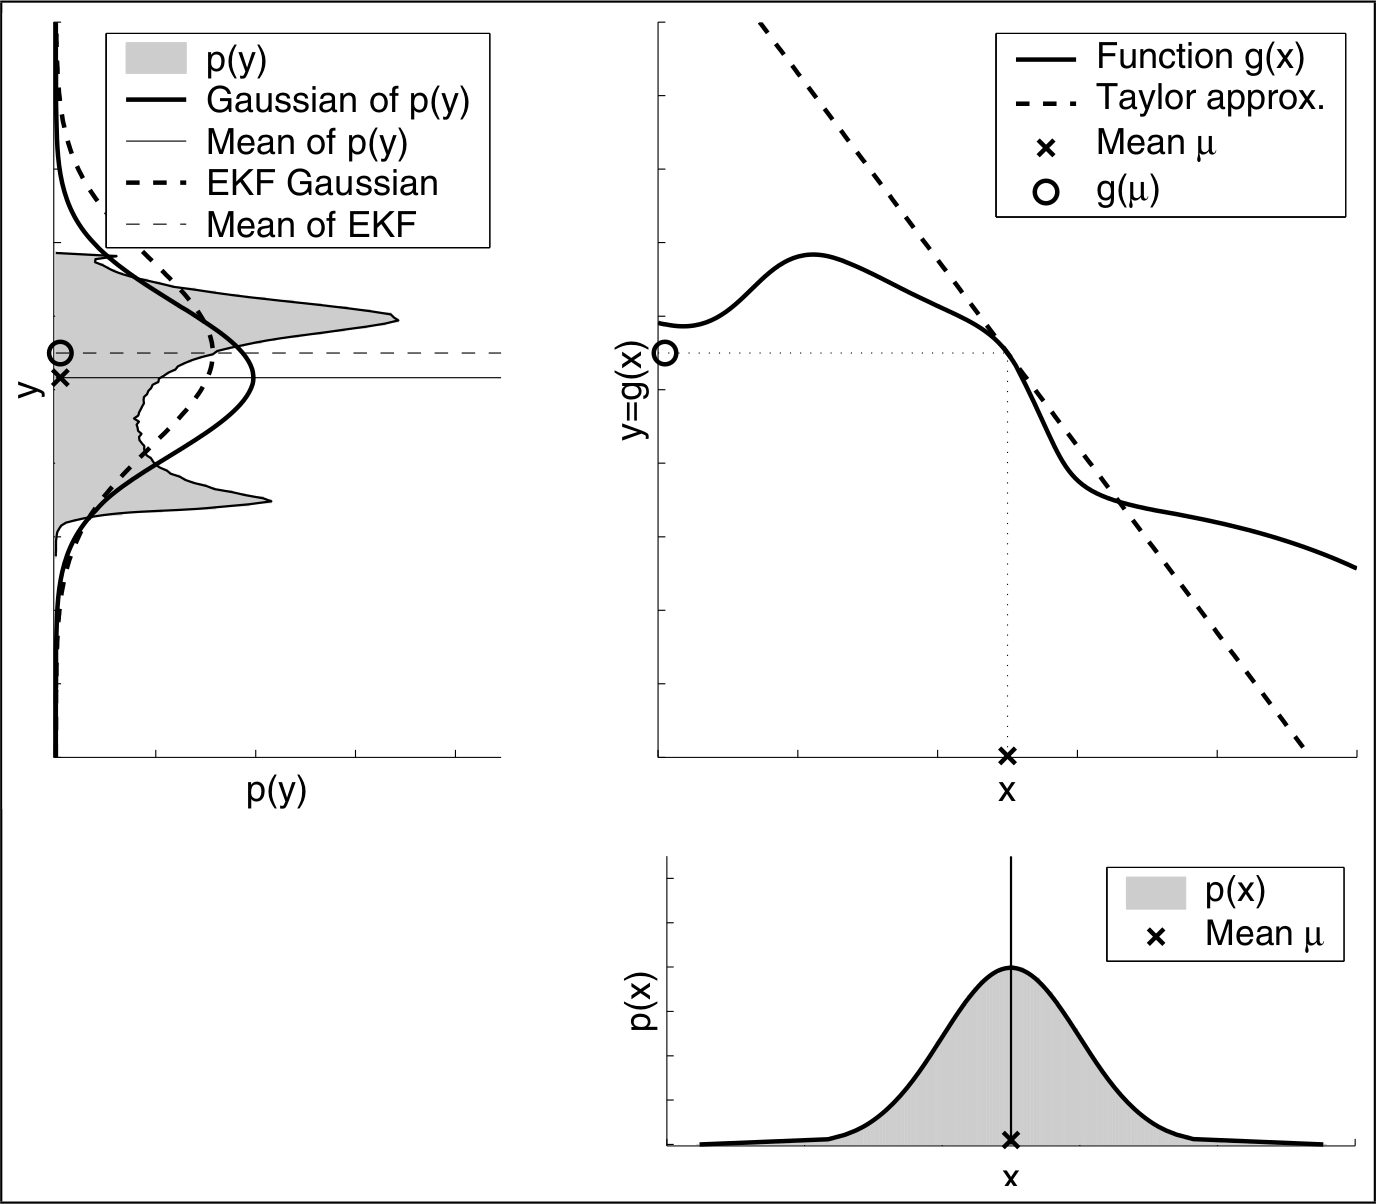
\includegraphics[width=\linewidth]{random_variable_taylor_linearization}
		\caption{}
		\label{fig:random_variable_taylor_linearization}
	\end{subfigure}
	\captionwithcite{Lineare und nicht lineare Transformation einer normalverteilten Zufallsvariable.}{\cite{thrun2005probabilistic}}
	\label{fig:random_variable_transformation}
\end{figure}


%%%%%%%%%%%%%%%%%%%%%%%%%%%%%%%%%%%%%%%%%%%%%%%%%%%%%%%%%%%%%%%%%%%%%%%%%%%%%%%%
%
% Belief: A belief reflects the robot’s internal knowledge about the state of the environment.
% Posterior:
%	- is the conditional probability that is assigned after the relevant evidence or background is taken into account.
% sample: Stichprobe, Abtasten
% a posteriori:
% a priori:
% non-parametric: parameterfreie, nichtparametrische, verteilungsfreie
% nonlinear transformations of random variables:
%
%%%%%%%%%%
\section{\glsentrylong{pf}}

Bisherige Filter haben eine parametrisierte Form genutzt, um die Verteilung zu modellieren. Der \Gls{pf} geht einen anderen Weg und verwendet stattdessen eine Menge von Stichproben (engl. Samples) aus der gewünschten Verteilung. Dadurch ist es möglich multimodale Verteilungen abzubilden, die jedoch nur einer Annäherung entsprechen. Weiterhin ist es möglich Zufallsvariablen durch eine nicht lineare Funktion abzubilden, siehe \autoref {fig:particle_filter_with_non_linear_function}. Im unteren rechten Bild wird eine Menge von Stichproben aus einer Normalverteilung dargestellt. Diese werden dann durch die nicht lineare Funktion $g(x)$ auf eine multimodale Verteilung abgebildet. Je dichter die Stichproben an einander liegen desto höher ist an dieser Stelle auch die Wahrscheinlichkeit.

\begin{figure}
	\centering
	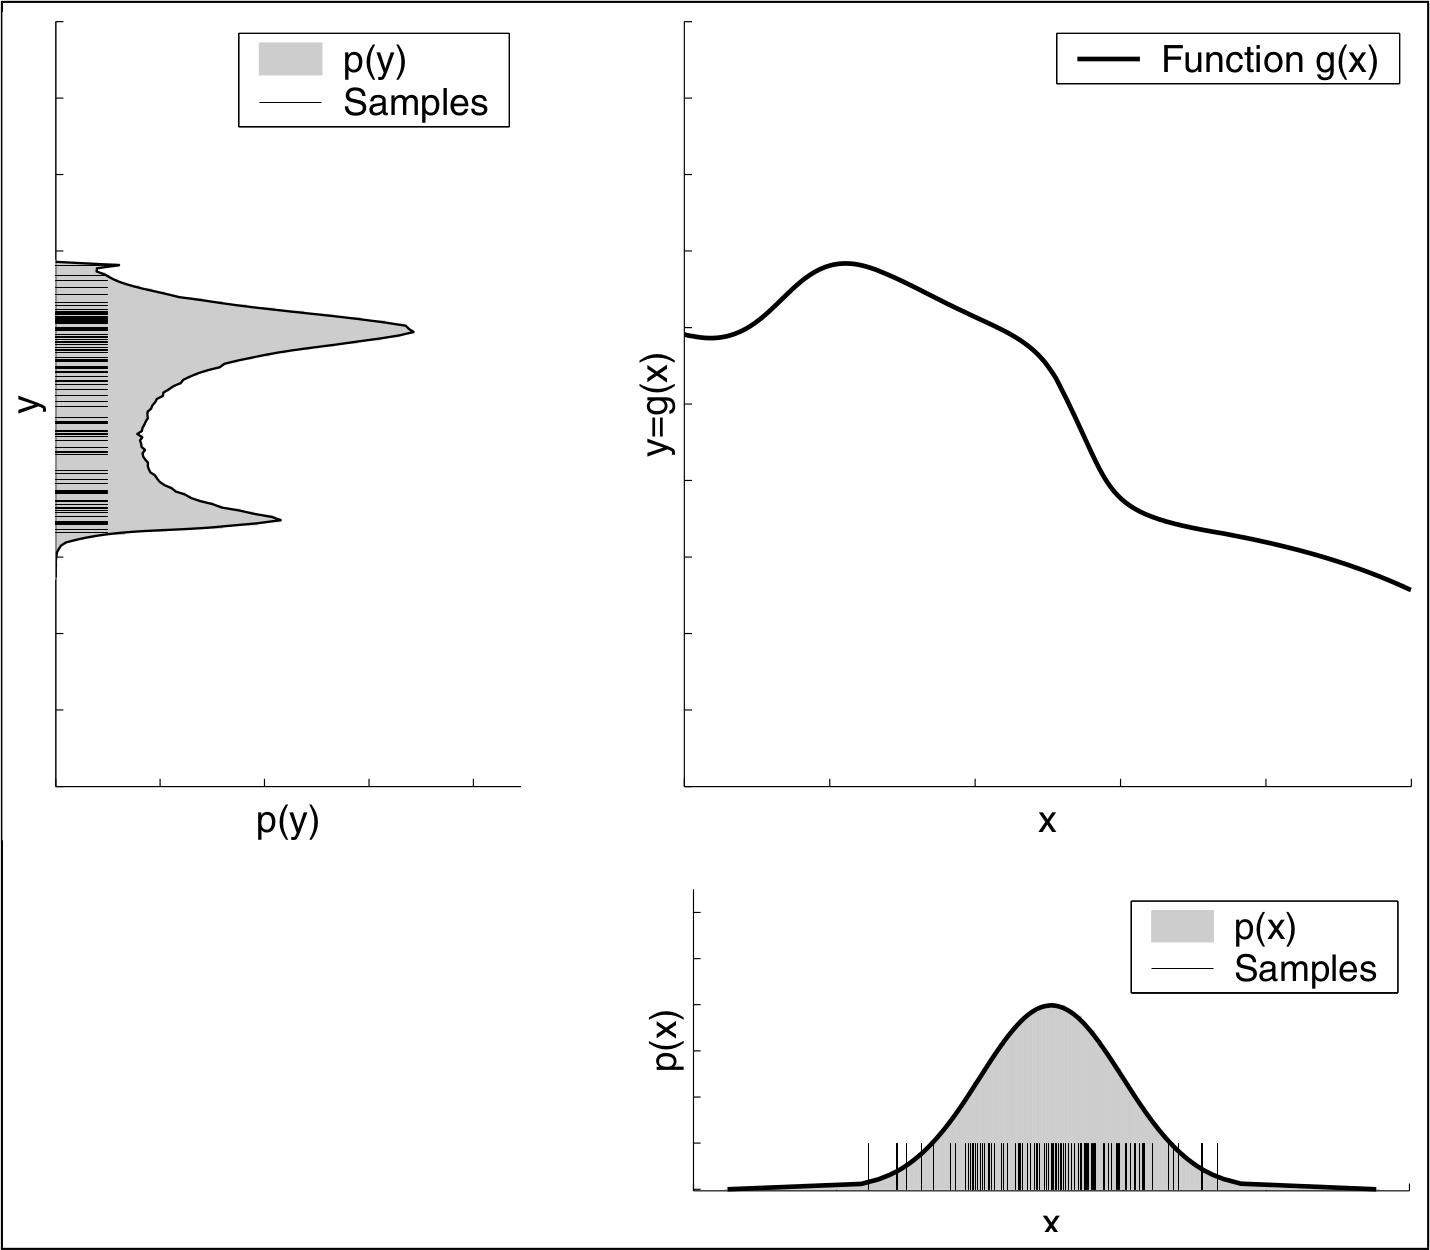
\includegraphics[width=0.6\linewidth]{particle_filter_with_non_linear_function}
	\captionwithcite{Darstellung einer Zufallsvariable vor und nach der Abbildung, durch eine nicht lineare Funktion, mittels einem \glsentrylong{pf}.}{\cite{thrun2005probabilistic}}
	\label{fig:particle_filter_with_non_linear_function}
\end{figure}

Die Stichproben aus der a posteriori Verteilung werden als Partikel (engl. Particle) bezeichnen. Jeder Partikel~$x_t$ entspricht dabei einer Hypothese des Weltzustandes zum Zeitpunkt~$t$. Über ein Gewicht~$w_t$ wird die Relevanz (engl. Importance Weight) eines Partikels ausgedrückt. Die Idee ist es dabei, durch ein Set von Partikeln den Belief~$bel(x_t)$ möglichst gut Anzunähern, siehe \autoref{eq:particle_filter_particle_set}. Der Parameter $M$ entspricht dabei der Anzahl der Partikel und wird sehr großzügig gewählt, z.B. $M=1000$.

\begin{equation}
\mathcal{X}_t := x^{\lbrack 1 \rbrack}_t, x^{\lbrack 2 \rbrack}_t, \ldots, x^{\lbrack M \rbrack}_t \label{eq:particle_filter_particle_set}
\end{equation}

Bei dem \Gls{pf} handelt es sich, wie bei dem Bayes Filter, ebenfalls um einen rekursiven Algorithmus, dem das vorherige Partikel-Set $\mathcal{X}_{t-1}$, die aktuellen Steuerbefehle $u_t$ und Wahrnehmungen $z_t$ übergeben werden, siehe \autoref{fig:algorithm_particle_filter}. Dabei wird im ersten Schritt auf jedem Partikel, aus dem vorherigen Set, die aktuellen Steuerbefehle angewendet und somit eine neue Prognose für den aktuellen Zustand gebildet, siehe Zeile 4. Weiterhin wird mit der neuen Zustandsprognose und den aktuellen Wahrnehmungen das Gewicht des Partikels bestimmt, siehe Zeile 5. Die aktuelle Zustandsprognose sowie das Gewicht werden danach in dem temporären Set $\overline{\mathcal{X}}_t$ gesammelt, siehe Zeile 6. Im zweiten Schritt findet das sogenannte \textit{Resampling} oder \textit{Importance Sampling} statt, siehe Zeile 9. Hierbei werden die Partikel mit einem hohen Gewicht beibehalten und die mit einem geringen durch neue ersetzt, die im Bereich der Partikel mit den hohen Gewichten liegen. Dadurch ist gewährleistet, dass sich die Partikel nicht in Bereichen mit einer geringen a posteriori Wahrscheinlichkeit aufhalten. Das Ergebnis aus dem letzten Schritt wird in dem Partikel-Set $\mathcal{X}_t$ gespeichert und dem Aufrufer zurückgegeben.

\begin{figure}
	\centering
	\fbox{	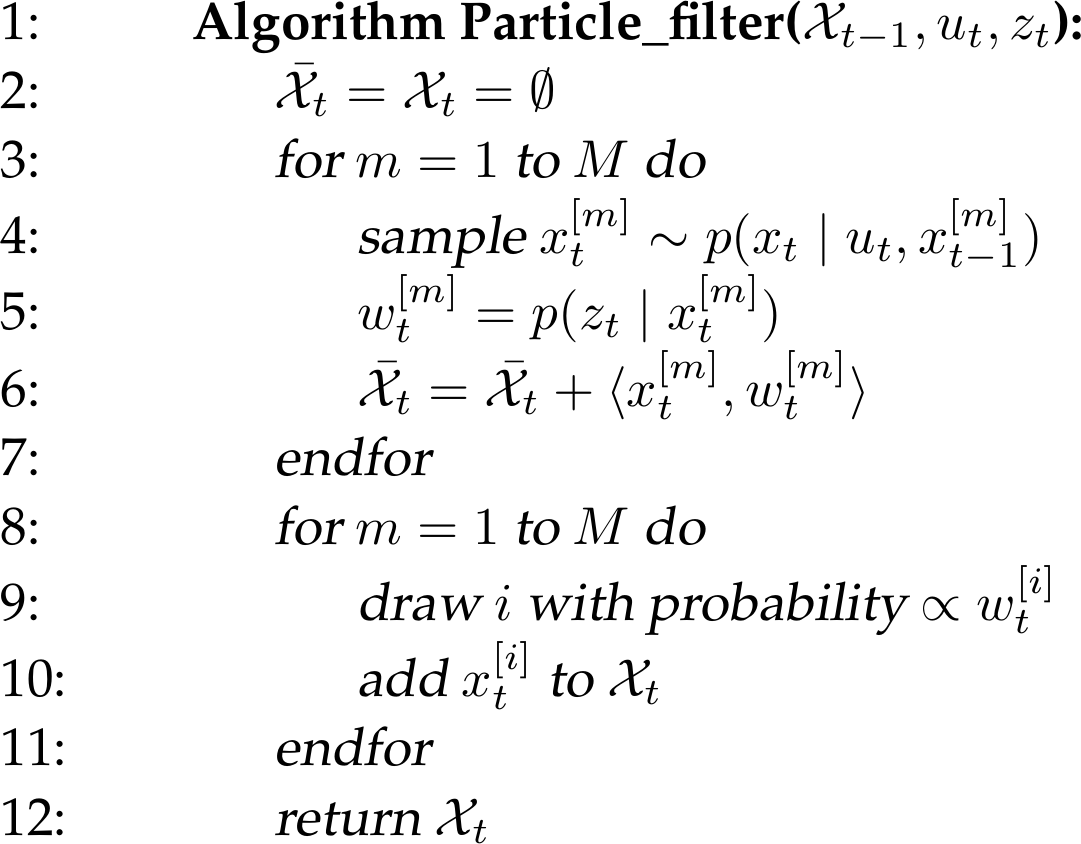
\includegraphics[width=0.5\linewidth]{algorithm_particle_filter}}
	\captionwithcite{\glsentrylong{pf} Algorithmus}{\cite{thrun2005probabilistic}}
	\label{fig:algorithm_particle_filter}
\end{figure}


%%%%%%%%%%%%%%%%%%%%%%%%%%%%%%%%%%%%%%%%%%%%%%%%%%%%%%%%%%%%%%%%%%%%%%%%%%%%%%%%
%
%	- \cite{kurth2003experimental}
%		- Monte Carlo localization, or particle filtering, provides a method of representing multimodal distri-butions for position estimation [4, 12], with the ad-vantage that the computational requirements can be scaled. The main advantage of these methods is their ability to recover robustly from a poor initial condition.
%	- \cite{fox1999monte}
%
%%%%%%%%%%
\subsection{\glsentrylong{mcl}}

Das Bestimmen der Pose eines Roboters relativ zu einer gegebenen Karte der Umwelt wird als Lokalisierung bezeichnet. Die Lokalisierung bestimmt dabei die Transformation zwischen dem lokalen Koordinatensystem des Roboters und dem globalen Koordinatensystem der Karte. Ist die initiale Pose des Roboters nicht gegeben, wird dieses Problem als globale Lokalisierung bezeichnet. Je größer die Karte der Umwelt ist, desto wahrscheinlicher wird es, dass die Wahrnehmung, Mehrdeutigkeiten in Bezug zu der Karte aufweist, die sich in einer multimodalen Verteilung wiederspiegeln und damit ideal durch einen \Gls{pf} abgebildet werden kann. Bei der \Gls{mcl} handelt es sich um genau so einen \Gls{pf}, der mittlerweile zu den Standardalgorithmen der Robotik gehört.

Die zwingende Voraussetzung, für die Lokalisierung, ist das vorhanden sein einer sehr genauen Karte der Umwelt. Die Kartendaten $m$ werden bei der Berechnung der Gewichte für die Zustandsprognosen eingesetzt. Somit unterscheidet sich der Monte Carlo Algorithmus nur in der fünften Zeile von dem generische Partikel Filter Algorithmus, siehe \autoref{eq:monte_carlo_measurement_model}. 

\begin{equation}
w^{\lbrack m \rbrack}_t = p(z_t \mid x^{\lbrack m \rbrack}_t, m) \label{eq:monte_carlo_measurement_model}
\end{equation}

% TODO: Erklären wie die MCL abläuft?
%
%- 8. Monte Carlo Localization
%	- Figure 8.11 - Monte Carlo Localization, a particle filter applied to mobile robot localization.
%	- The initial global uncertainty is achieved through a set of pose particles drawn at random and uniformly over the entire pose space, as shown in Figure 8.11a.
%	- As the robot senses the door, MCL assigns importance factors to each particle. The resulting particle set is shown in Figure 8.11b.
%	- The height of each particle in this figure shows its importance weight.
%	- It is important to notice that this set of particles is identical to the one in Figure 8.11a—the only thing modified by the measurement update are the importance weights.
%	- Figure 8.11c shows the particle set after resampling and after incorporating the robot motion. This leads to a new particle set with uniform importance weights, but with an increased number of particles near the three likely places.
%	- The new measurement assigns non-uniform importance weights to the particle set, as shown in Figure 8.11d.
%	- At this point, most of the cumulative probability mass is centered on the second door, which is also the most likely location.

%\begin{figure}
%	\centering
%	\begin{subfigure}{0.8\linewidth}
%		\centering
%		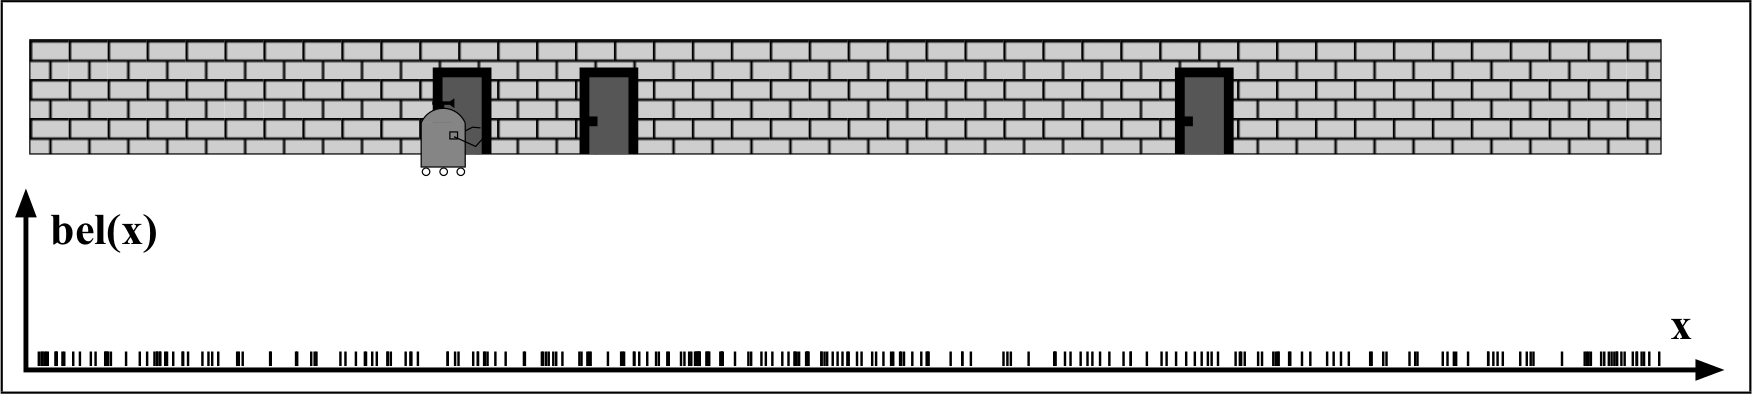
\includegraphics[width=\linewidth]{thrun2005probabilistic_fig811a}
%		\caption{}
%		\label{fig:thrun2005probabilistic_fig811a}
%	\end{subfigure}
%	\par\bigskip
%	\begin{subfigure}{0.8\linewidth}
%		\centering
%		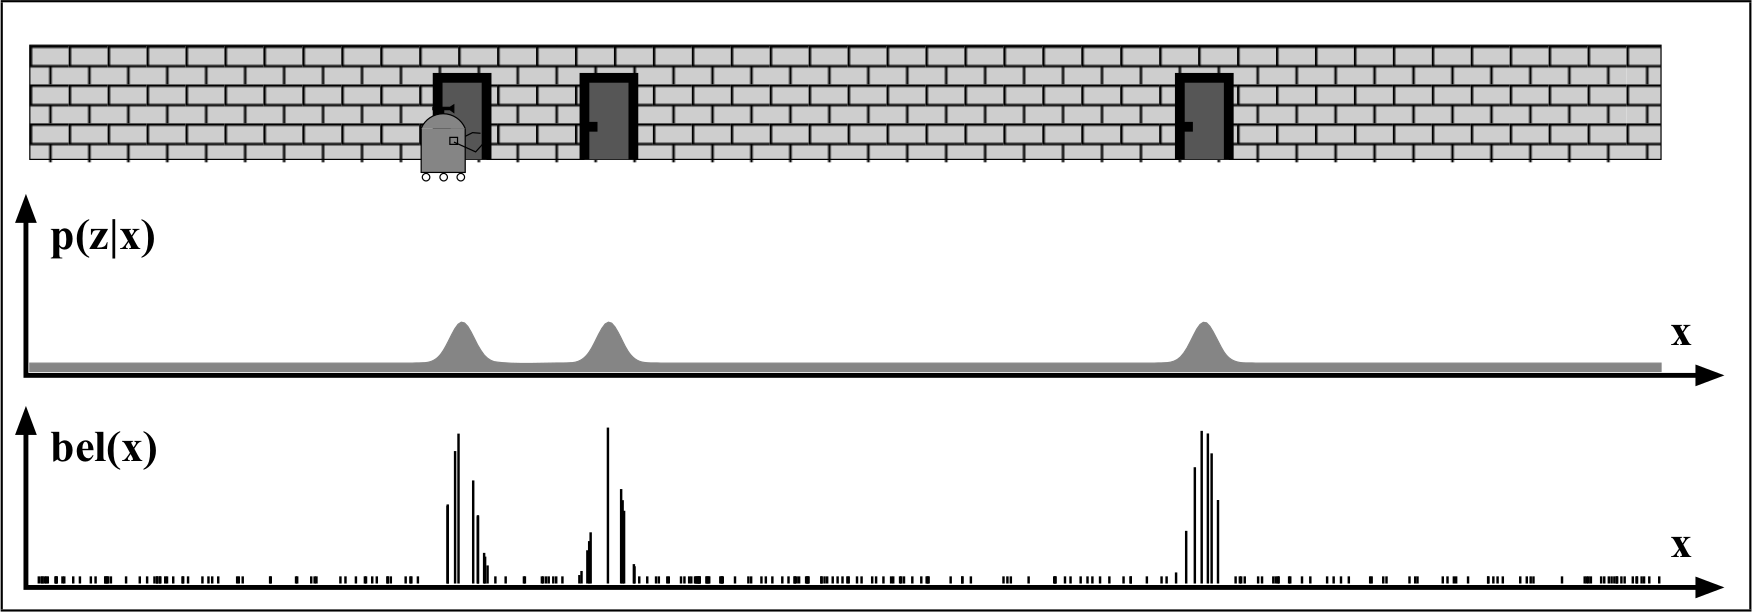
\includegraphics[width=\linewidth]{thrun2005probabilistic_fig811b}
%		\caption{}
%		\label{fig:thrun2005probabilistic_fig811b}
%	\end{subfigure}
%	\par\bigskip
%	\begin{subfigure}{0.8\linewidth}
%		\centering
%		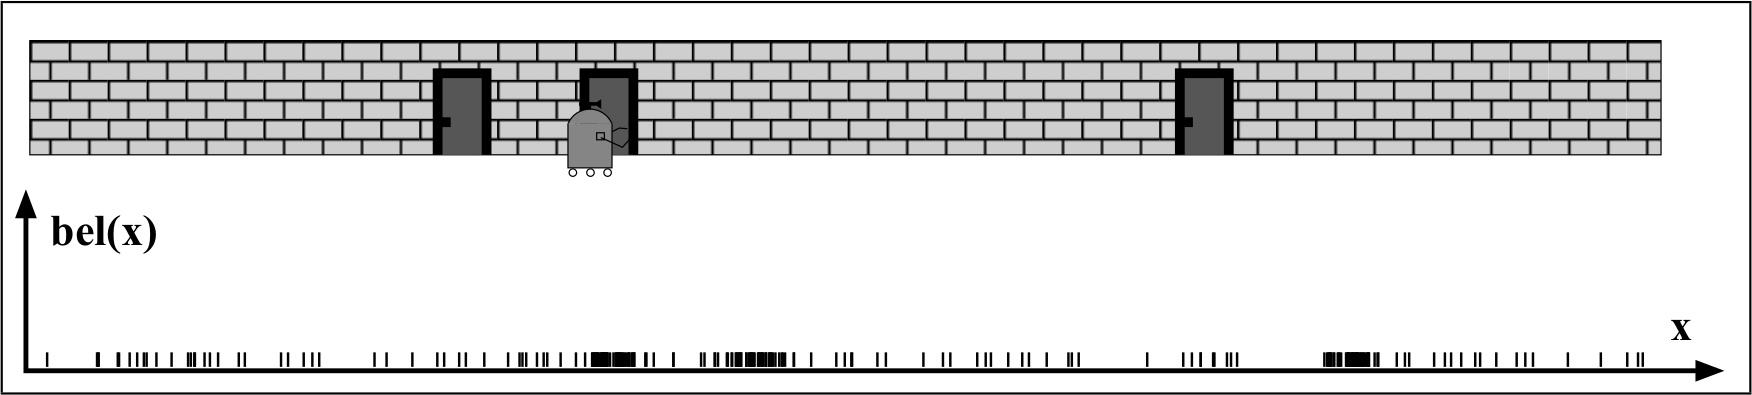
\includegraphics[width=\linewidth]{thrun2005probabilistic_fig811c}
%		\caption{}
%		\label{fig:thrun2005probabilistic_fig811c}
%	\end{subfigure}
%	\par\bigskip
%	\begin{subfigure}{0.8\linewidth}
%		\centering
%		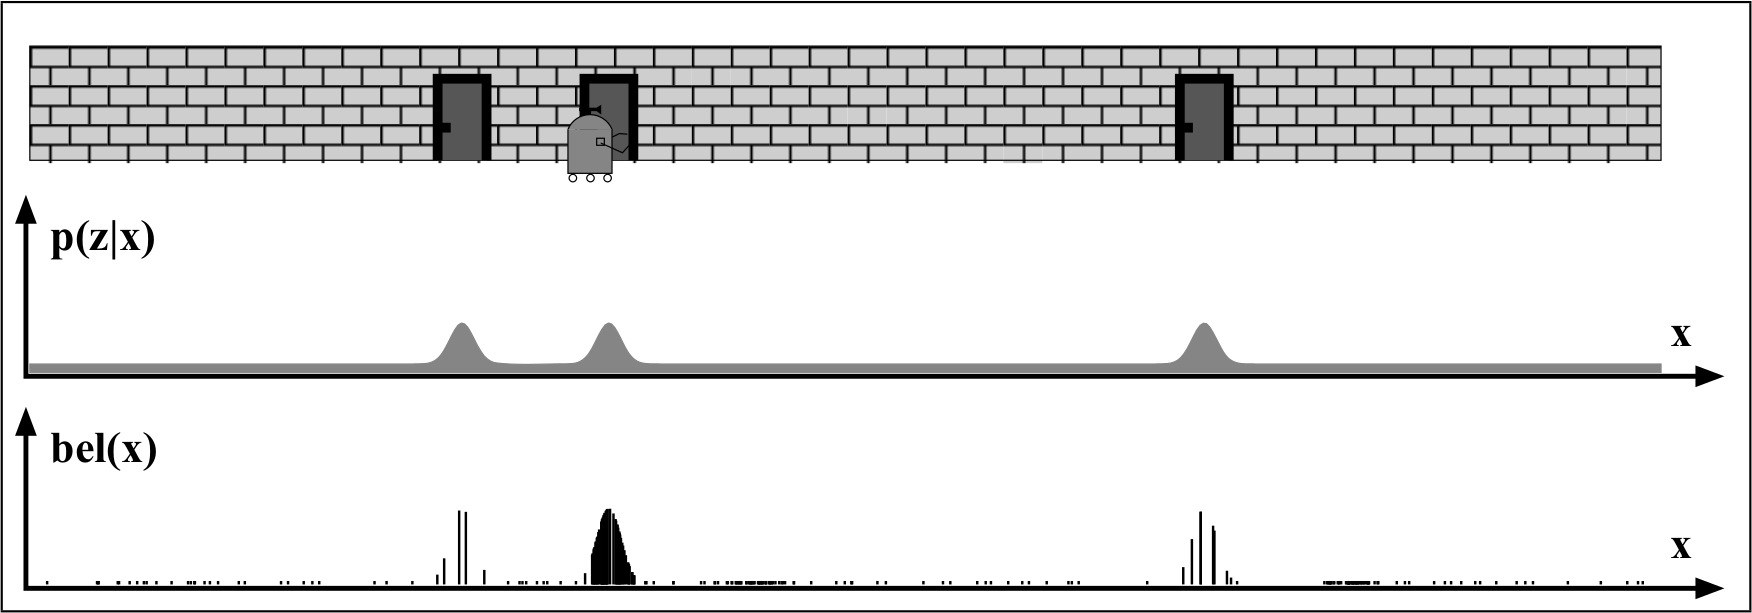
\includegraphics[width=\linewidth]{thrun2005probabilistic_fig811d}
%		\caption{}
%		\label{fig:thrun2005probabilistic_fig811d}
%	\end{subfigure}
%	\par\bigskip
%	\begin{subfigure}{0.8\linewidth}
%		\centering
%		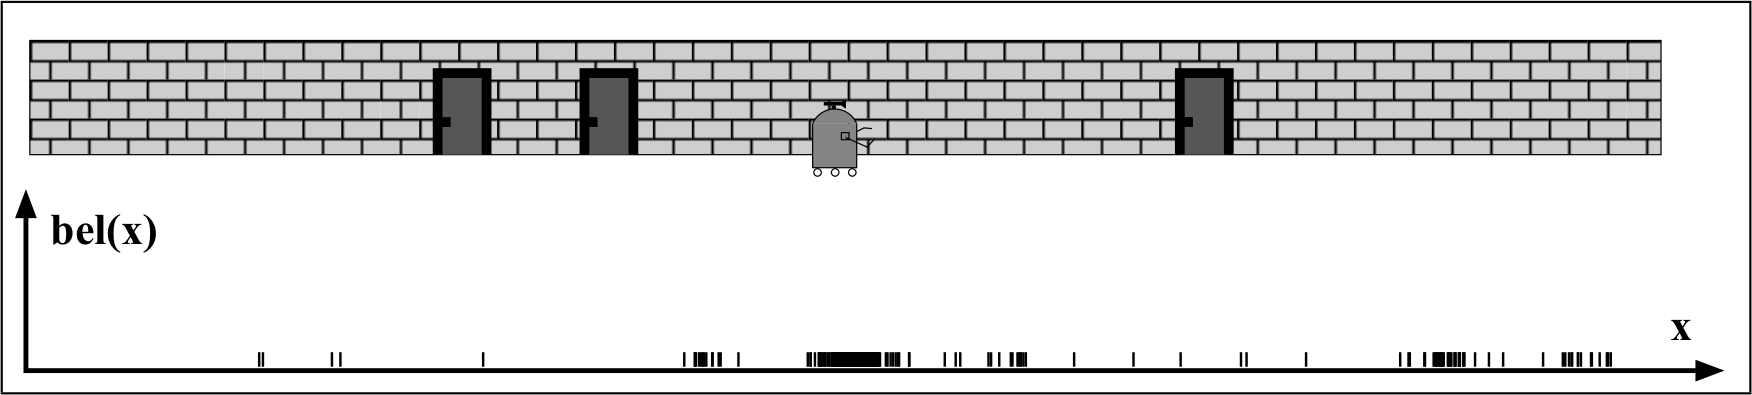
\includegraphics[width=\linewidth]{thrun2005probabilistic_fig811e}
%		\caption{}
%		\label{fig:thrun2005probabilistic_fig811e}
%	\end{subfigure}
%	\captionwithcite{Beispiel für die Positionsbestimmung eines Roboter mittels der \glsentrylong{mcl}.}{\cite{thrun2005probabilistic}}
%	\label{fig:thrun2005probabilistic_fig811}
%\end{figure}


%%%%%%%%%%%%%%%%%%%%%%%%%%%%%%%%%%%%%%%%%%%%%%%%%%%%%%%%%%%%%%%%%%%%%%%%%%%%%%%%
%
% 	- \cite{kurth2003experimental}
%		- We are currently developing a batch localization method, which considers all the data collected by the robot and finds the best path estimate given all the data. Although time consuming computationally, this will produce the theoretically optimal result obtainable from the collected data; we can then evaluate the results of our online localization method by comparing to this optimal solution.
%	- \cite{}
%		- Comparison of Batch and Kalman Filtering for Radar Tracking
%		- http://www.dtic.mil/dtic/tr/fulltext/u2/p011192.pdf
%		- The EKF propagates the filter state between measurements, and incorporates measurements sequentially, with the error dynamics and observation models respectively. It is an implementation of the often referenced linear-minimum-variance (Kalman) formulas, adapted by first-variation approximations of the nonlinear models, centered at the current state estimate, and described in Reference [4] (Jazwinski). 	
%		- The Batch algorithm, in comparison, processes those same measurements simultaneously via iterative least-squares estimation. An overview of the comparison of measurement processing among the two algorithms is shown in Figure-1. Batch algorithm estimations were made in parallel with those of the EKF for comparison of estimation error time histories.
%
%%%%%%%%%%
%\section{Batch optimization [todo,optional]}


%%%%%%%%%%%%%%%%%%%%%%%%%%%%%%%%%%%%%%%%%%%%%%%%%%%%%%%%%%%%%%%%%%%%%%%%%%%%%%%%
%
%	- \cite{kurth2003experimental}
%		- Additionally, we will extend the batch method to produce a variable dimension filter, as used by Deans for the case of bearing-only sensors [3], which would consider some window of previous robot states and optimize the position estimates based on the data in that window.
%
%%%%%%%%%%
%\section{Variable Dimension Filter [todo,optional]}


%%%%%%%%%%%%%%%%%%%%%%%%%%%%%%%%%%%%%%%%%%%%%%%%%%%%%%%%%%%%%%%%%%%%%%%%%%%%%%%%
%
%	- SLAM
%		- Verwenden der Sensordaten um sich zu Lokalisierung...
%		- und eine Karte der Landmarken zu erzeugen.
%		- Bisher Winkel und Entferung zu einer Landmarke gegeben
%			- Computer Vision, Structure from Motion
%	- Embodied Localisation and Mapping
%		- http://elib.suub.uni-bremen.de/edocs/00103537-1.pdf
%
%%%%%%%%%%
\section{\glsentrylong{slam}}


% Was versteht man unter Mapping?
%- a priori map
%- And even if blueprints were accurate, they would not contain furniture and other items that, from a robot’s perspective, determine the shape of the environment just as much as walls and doors. Being able to learn a map from scratch can greatly reduce the efforts involved in installing a mobile robot, and enable robots to adapt to changes without human supervision
%- In this chapter, we first study the mapping problem under the restrictive assumption that the robot poses are known.
%	- is also known as mapping with known poses.
%	- Occupancy grid mapping addresses the problem of generating consistent maps from noisy and uncertain measurement data, under the assumption that the robot pose is known.
%	- The basic idea of the occupancy grids is to represent the map as a field of random variables, arranged in an evenly spaced grid. Each random variable is binary and corresponds to the occupancy of the location it covers. Occupancy grid mapping algorithms implement approximate posterior estimation for those random variables.


% Was versteht man unter SLAM?
Wenn der Roboter weder seine eigne Pose kennt noch eine Karte seiner Umwelt besitzt, beides jedoch aus den Steuerbefehlen $u_{1:t}$ und den Wahrnehmungen $z_{1:t}$ bestimmen soll, wird das als \Gls{slam}\footnotemark{} Problem bezeichnet. 

\footnotetext{Alternativ zu \acrfull{slam} wird auch \acrfull{cml} verwendet.}

% Unterschied zwischen Online/Full SLAM? {Graph-Modell, Eqaution}
Es gilt dabei zu unterscheiden zwischen dem Online- und Full-\gls{slam}. Beim Online-\gls{slam} wird die aktuelle Pose $x_t$ innerhalb der Karte geschätzt, siehe \autoref{eq:online_slam_problem}, während beim Full-\gls{slam} die komplette Trajektorie $x_{1:t}$ innerhalb der Karte geschätzt wird, siehe \autoref{eq:full_slam_problem}.

\begin{equation}
p(x_t, m \mid z_{1:t}, u_{1:t}) \label{eq:online_slam_problem}
\end{equation}

\begin{equation}
p(x_{1:t}, m \mid z_{1:t}, u_{1:t}) \label{eq:full_slam_problem}
\end{equation}

%\begin{figure}
%	\centering
%	\begin{subfigure}{0.4\linewidth}
%		\centering
%		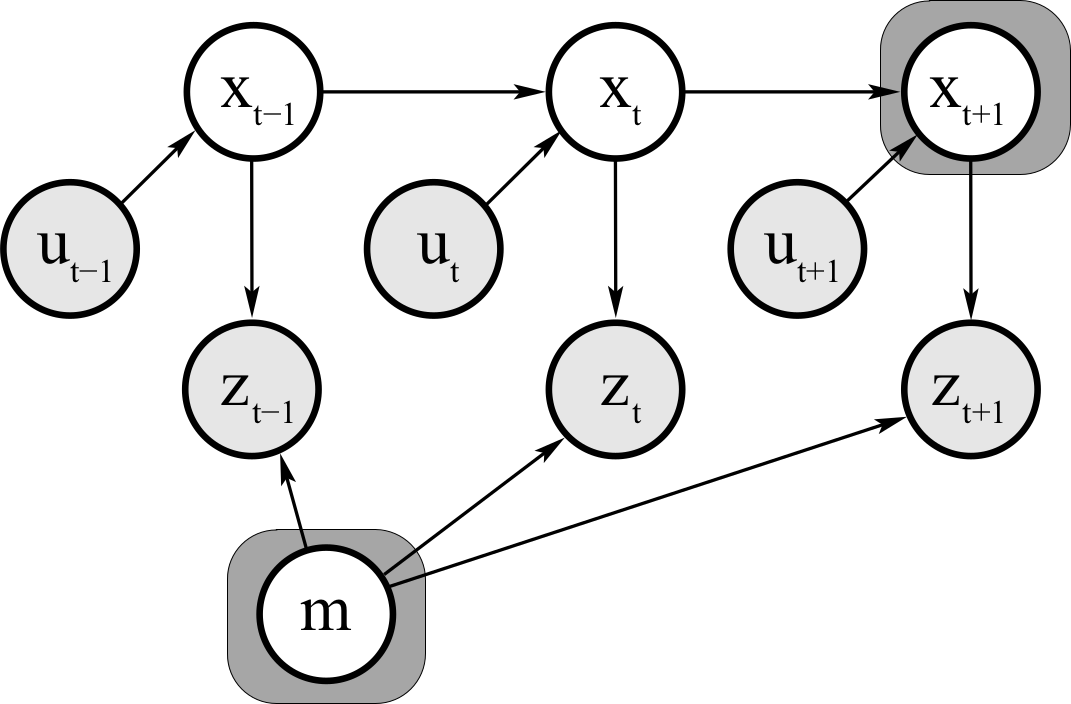
\includegraphics[width=\linewidth]{thrun2005probabilistic_fig10_1}
%		\caption{}
%		\label{fig:thrun2005probabilistic_fig10_1}
%	\end{subfigure}
%	\hfill
%	\begin{subfigure}{0.4\linewidth}
%		\centering
%		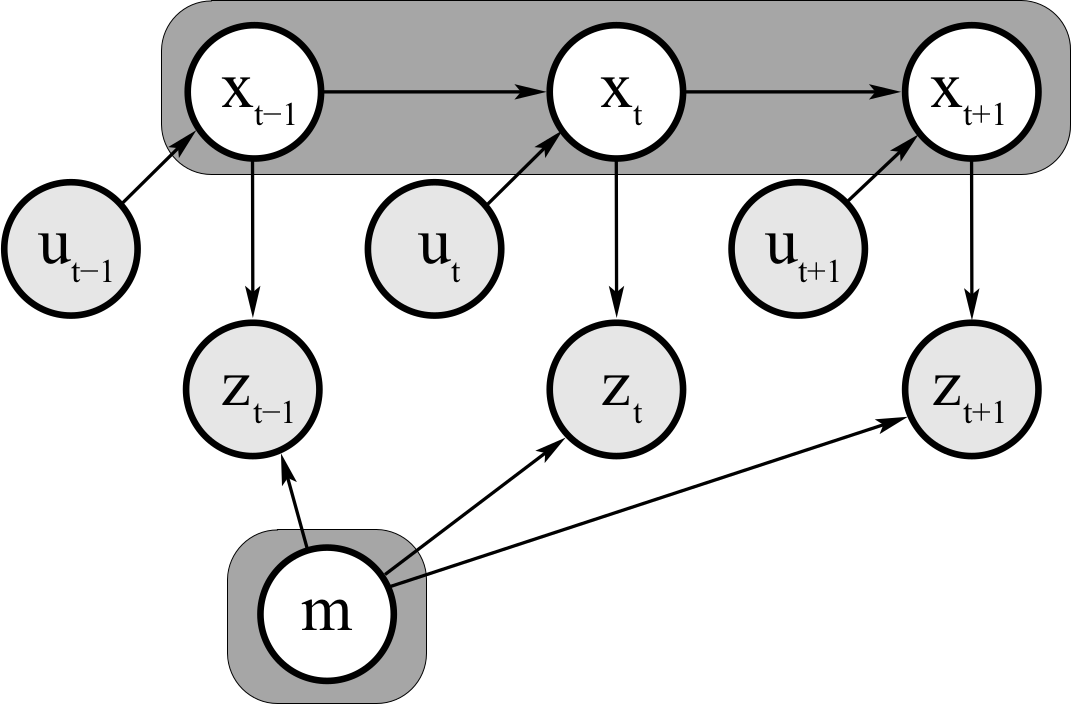
\includegraphics[width=\linewidth]{thrun2005probabilistic_fig10_2}
%		\caption{}
%		\label{fig:thrun2005probabilistic_fig10_2}
%	\end{subfigure}
%	\captionwithcite{Die graphischen Modelle für den Online- bzw. Full-\gls{slam}.}{\cite{thrun2005probabilistic}}
%	\label{fig:thrun2005probabilistic_fig10_1_2}
%\end{figure}


%%%%%%%%%%%%%%%%%%%%%%%%%%%%%%%%%%%%%%%%%%%%%%%%%%%%%%%%%%%%%%%%%%%%%%%%%%%%%%%%
%
%
%
%%%%%%%%%%
\subsection{EKF-SLAM}

% Warum gerade SLAM mit EKF?
Eine der ersten Implementierung des Online-\gls{slam} Algorithmus wurde auf der Basis des \gls{ekf} durchgeführt. Neben der Pose des Roboters, werden auch alle Position der wahrgenommenen Landmarken geschätzt. Somit besteht die Karte der Umwelt aus allen Positionen der Landmarken und wird daher auch als merkmalsbasierte Karte (engl. Feature-Based Map) bezeichnet.

% Wie sieht der Zustandsvektor aus?
Bisher bestand der Zustandsvektor aus den drei Komponenten X-/Y-Position und der Orientierung $\theta$ um die Pose des Roboters zu beschreiben. Für den EKF-SLAM wird der Zustandsvektor um die X-/Y-Position der vorhandenen Landmarken erweitert, siehe \autoref{eq:ekf_slam_state_vector}. Diese Kombination aus Pose des Roboters und Positionen der Landmarken wird als kombinierter Zustandsvektor (engl. Combined State Vector) bezeichnet.

\begin{equation}
x_t = \left( x, y, \theta, m_{1,x}, m_{1,y}, \ldots, m_{n,x}, m_{n,y} \right)^T \label{eq:ekf_slam_state_vector}
\end{equation}

% Wie sieht die Modellierung für den Belief mit mean und covarianz aus?
Um den \gls{ekf} einsetzten zu können, muss der Belief mittels der beiden Momente $\mu$ und $\Sigma$ beschrieben werden. $\mu$ entspricht dabei dem kombinierte Zustandsvektor $x_t$ und $\Sigma$ beschreibt die Unsicherheiten der Roboter Pose, der Landmarken Positionen und die Unsicherheit zwischen der Roboter Pose und den Landmarken Positionen, siehe \autoref{eq:ekf_slam_mu_sigma}.

\begin{equation}
\mu = \begin{pmatrix} x_R \\ m_1 \\ \vdots \\ m_n \end{pmatrix}
\qquad
\Sigma = \begin{pmatrix}
	\Sigma_{x_R x_R} & \Sigma_{x_R m_1} & \cdots & \Sigma_{x_R m_n} \\
	\Sigma_{m_1 x_R} & \Sigma_{m_1 m_1} & \cdots & \Sigma_{m_1 m_n} \\
	\vdots & \vdots & \ddots & \vdots \\
	\Sigma_{m_n x_R} & \Sigma_{m_n m_1} & \cdots & \Sigma_{m_n m_n}
\end{pmatrix}
\label{eq:ekf_slam_mu_sigma}
\end{equation}

% Welche Einschränkungen ergeben sich für den EKF-SLAM?
Bei der Verwendung des EKF-SLAM ist zu berücksichtigen, dass die Wahrnehmungsdaten möglichst eindeutig den Landmarken zugeordnet werden können. Die Zuordnung kann dabei explizit gegeben sein oder durch einen zusätzlichen Algorithmus möglich gut geschätzt werden. Mehrdeutige Zuordnungen führen zu einem deutlich schlechteren Ergebnis.

Eine weitere Einschränkt betrifft die maximale Anzahl der Landmarken, da die Laufzeit und die Größe der Karte quadratisch mit der Anzahl der Landmarken wäschst.


%%%%%%%%%%%%%%%%%%%%%%%%%%%%%%%%%%%%%%%%%%%%%%%%%%%%%%%%%%%%%%%%%%%%%%%%%%%%%%%%
%
%	- Rao-Blackwellized Particle Filtering
%		- https://people.eecs.berkeley.edu/~pabbeel/cs287-fa12/slides/RBPF.pdf
%	- \cite{murphy2001rao}
%		- Rao-Blackwellised particle filtering for dynamic Bayesian networks
% 	- Model the robot's path by sampling and compute the landmarks given the pose
% 		- each particle represents a possible trajectory of the robot
% 		- each particle maintains its own map (2d ekf)
% 		- each particle updates it upon <mapping with known poses>
%	- If we use the particle set only to model the robot’s path, each sample is a path hypothesis.
%		- For each sample, we can compute an individual map of landmarks.
%		- Apply mapping with known poses
%	- Rao-Blackwellized particle filters use particles to represent the posterior over some variables, along with Gaussians (or some other parametric PDF) to represent all other variables.
%		- if an oracle told us the true robot path, we could estimate the location of all features independently of each other.
%		- Dependencies in these estimates arise only through robot pose uncertainty.
%		- This structural observation will make it possible to apply a version of particle filters to SLAM known as Rao-Blackwellized particle filters.
%
%%%%%%%%%%
\subsection{FastSLAM}

% Wie könnte das SLAM Problem mit einem PF gelöst werden? Wie sieht die Partikel repräsentation aus?
Bei dem \textit{FastSLAM} Verfahren handelt es sich um eine Lösung für das \gls{slam} Problem mithilfe eines \gls{pf}. Bei einem \gls{pf} repräsentiert jedes Partikel eine eigene Hypothese  des jeweiligen Zustandes des Roboters. Um das \gls{slam} Problem zu lösen muss der Zustandsvektor, wie beim EKF-SLAM, um die Landmarken erweitert werden, siehe \autoref{eq:ekf_slam_state_vector}.

% Was ist das Problem eines Partikel Filter mit dem SLAM Problem?
\gls{pf} haben jedoch die Eigenschaft, nur mit einem kleinen Zustandsraum gut zu funktionieren. Bei einem großen Zustandsraum werden deutlich mehr Stichproben benötigt, um diesen möglichst gut abzudecken. Der Aufwand skaliert dabei exponentiell mit der Anzahl der Dimensionen des Zustandsraumes, sodass eine praktikable Anwendung eines \gls{pf} nicht mehr gegeben ist.

% Was ist die Schlüsselidee?
Die Lösung des Problems besteht darin, mit dem \gls{pf} nur den Pfad des Roboters zu modellieren und dann für jede Pfadhypothese eine separate Karte der Umwelt mit ihren Landmarken zu berechnen.

% Was ist der RBPF?
Um die Berechnung der Karte von dem Pfad des Roboters zu trennen, wird der Umstand ausgenutzt, das beide Zufallsvariablen ein Wissen über einander besitzt. Dazu wird die \autoref{eq:conditional_probability}, für die bedingte Wahrscheinlichkeit, nach der multivariaten Verteilung umgestellt, siehe \autoref{eq:pf_slam_conditional_probability}. Anstatt nun die Verteilung sowohl für den Pfad des Roboters als auch den der Karte $p(x, y)$ zu bestimmen, wird die Verteilung nur für den Pfad des Roboters $p(x)$ bestimmt und dann für jede Pfadhypothese die sich daraus ergebende Karte $p(y \mid x)$ berechnet. Dieses Verfahren wird auch als \textit{Rao-Blackwellisierung} bezeichnet.

\begin{equation}
p(x, y) = p(y \mid x) \, p(x) \label{eq:pf_slam_conditional_probability}
\end{equation}

Das vorherige Verfahren wird nun auf die a posteriori Verteilung des \gls{slam} Problems übertragen, siehe \autoref{eq:pf_slam_posterior}. $x_{0:t}$ entspricht dabei den Pfad des Roboters, $m_{1:M}$ der Karte, $z_{1:t}$ den Wahrnehmungen und $u_{1:t}$ den Steuerbefehlen. Die ausfaktorisierten Terme $p(x_{0:t} \mid z_{1:t}, u_{1:t})$ und $p(m_{1:M} \mid x_{0t:t}, z_{1:t})$ bilden dabei die a posteriori Verteilung für den Pfad des Roboters und für die Karte der Umwelt.

\begin{equation}
p(x_{0:t}, m_{1:M} \mid z_{1:t}, u_{1:t}) = p(x_{0:t} \mid z_{1:t}, u_{1:t}) \, p(m_{1:M} \mid x_{0:t}, z_{1:t}) \label{eq:pf_slam_posterior}
\end{equation}

Der Term für die a posteriori Verteilung der Karte aus der \autoref{eq:pf_slam_posterior} kann noch optimiert werden. Dadurch das der Pfad des Roboters bekannt ist, gibt es keine Landmarke die über eine unbekannte Zufallsvariable mit einer anderen Landmarke verbunden ist, siehe \autoref{fig:fast_slam_conditionally_independent}. Das bedeutet, dass die Landmarken untereinander als unabhängige Zufallsvariable dargestellt werden können. Somit kann die a posteriori Verteilung der Karte als Produkt ihrer einzelnen Landmarken ausgedrückt werden, siehe \autoref{eq:pf_slam_optimized_posterior}. Dadurch kann jede Landmarke durch einen $2 \times 2$ großen \gls{ekf} modelliert und dadurch sehr effizient berechnet werden. Die Repräsentation des endgültigen Partikel kann der \autoref{fig:fast_slam_particle_representation} entnommen werden.

\begin{figure}
	\centering
	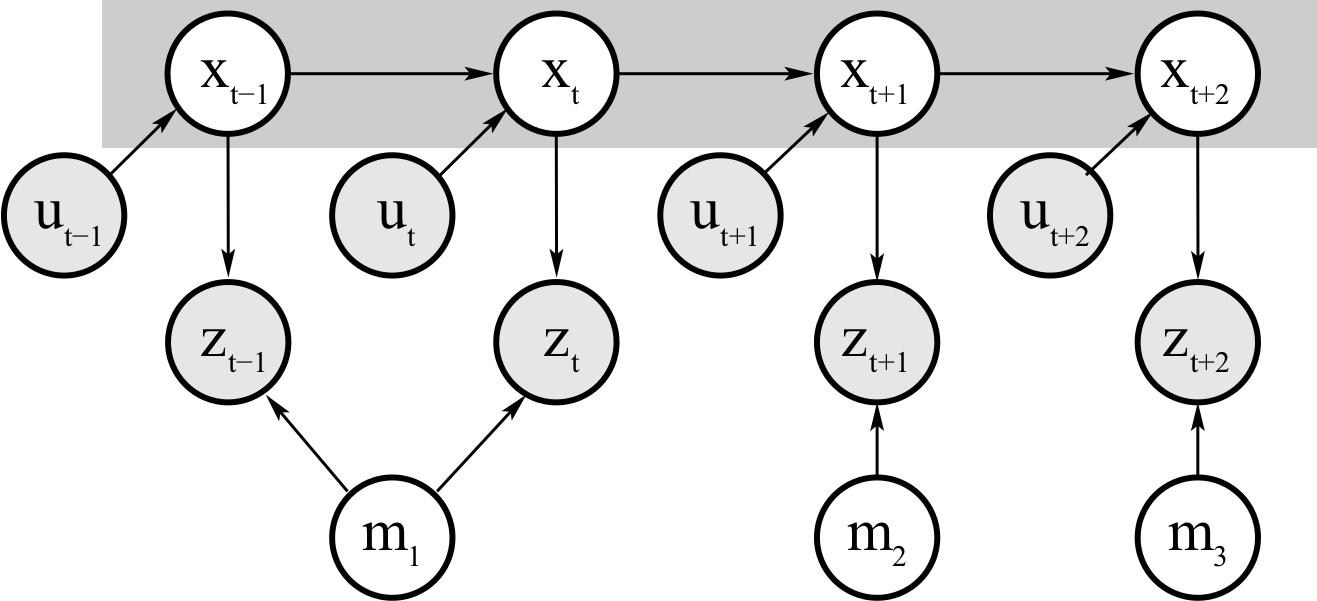
\includegraphics[width=0.5\linewidth]{fast_slam_conditionally_independent}
	\captionwithcite{Darstellung des \gls{slam} Problems als bayessches Netz.}{\cite{thrun2005probabilistic}}
	\label{fig:fast_slam_conditionally_independent}
\end{figure}

\begin{equation}
p(x_{0:t}, m_{1:M} \mid z_{1:t}, u_{1:t}) = p(x_{0:t} \mid z_{1:t}, u_{1:t}) \, \prod_{i=1}^{M} p(m_i \mid x_{0:t}, z_{1:t}) \label{eq:pf_slam_optimized_posterior}
\end{equation}

\begin{figure}
	\centering
	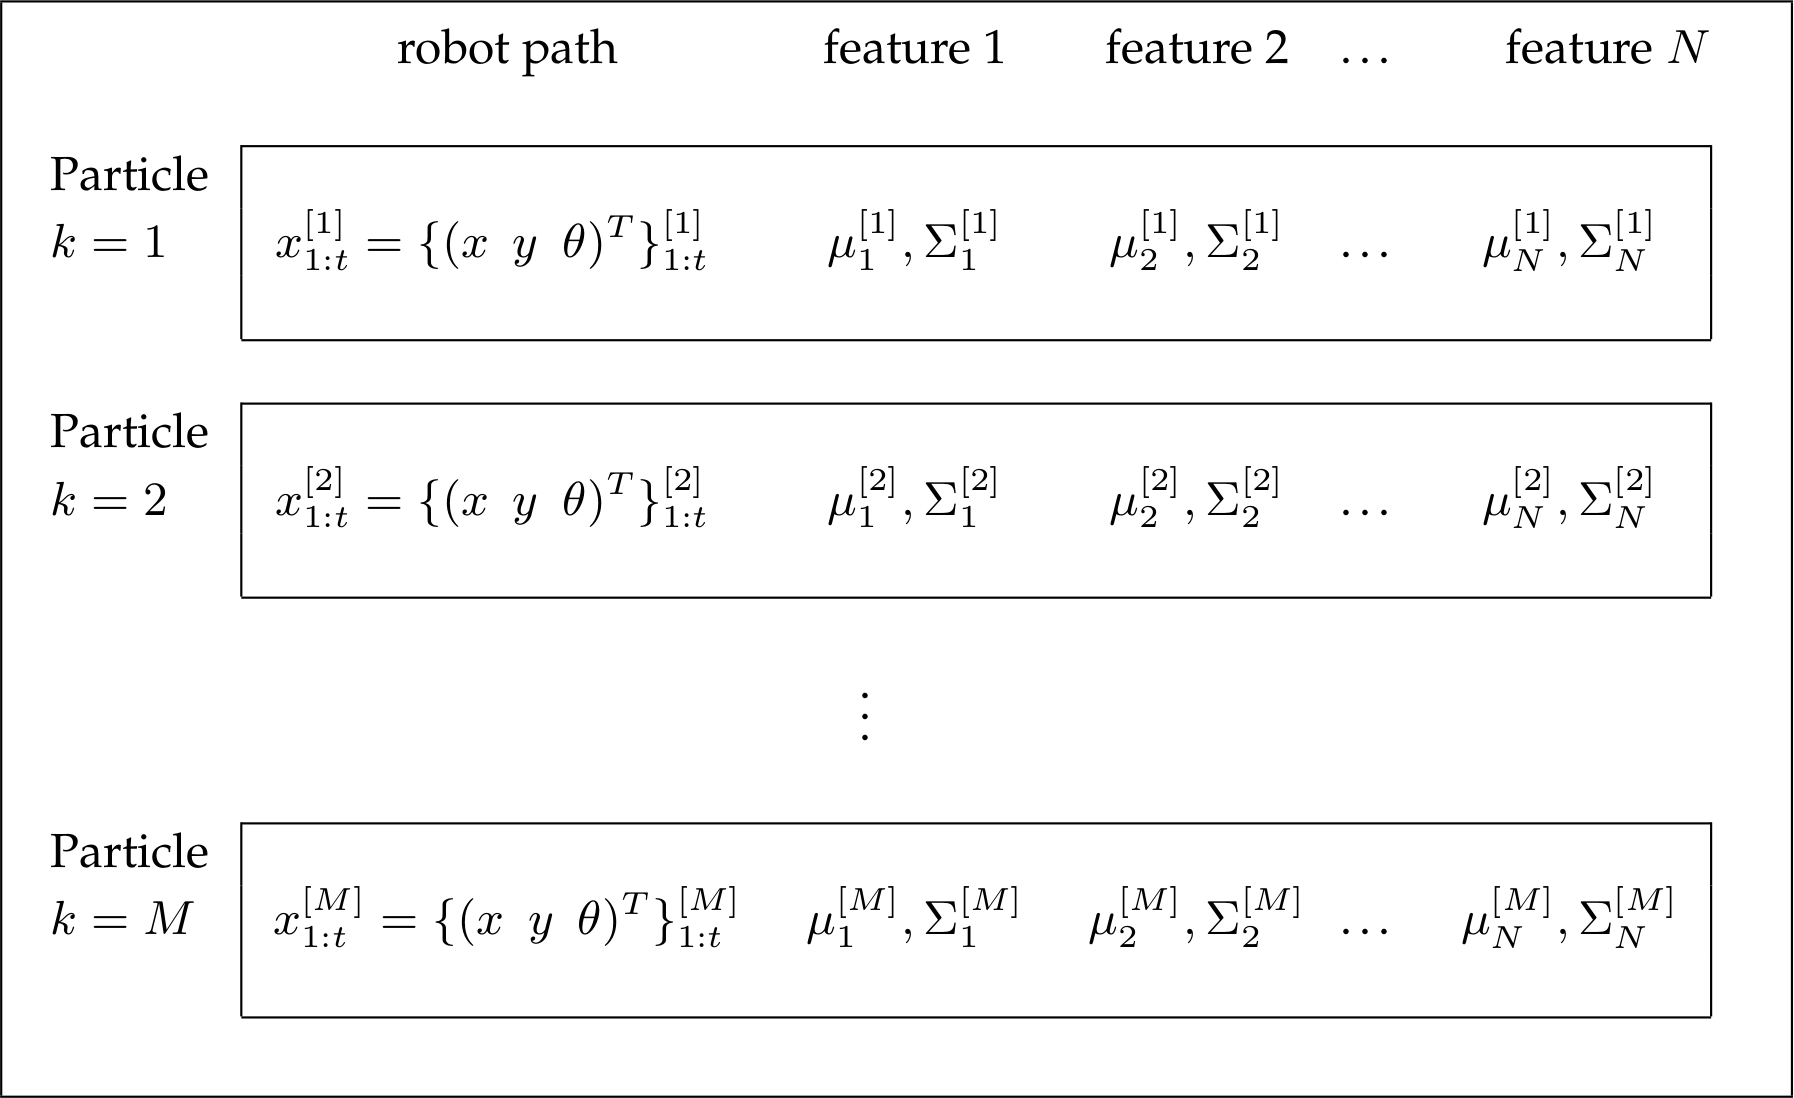
\includegraphics[width=0.7\linewidth]{fast_slam_particle_representation}
	\captionwithcite{Representation der Partikel in FastSLAM.}{\cite{thrun2005probabilistic}}
	\label{fig:fast_slam_particle_representation}
\end{figure}

Die Gewichte eines Partikels spielen eine große Rolle im \textit{Resampling} Prozess. Beim \textit{FastSLAM} entsteht die Gewichtung dabei aus der Erkenntnis, wie gut die Landmarken einer Pfadhypothese mit den Wahrnehmungen übereinstimmen.

Für den EKF-SLAM ist es entscheiden, die Zuordnung zwischen den Landmarken und den Wahrnehmungen zu kennen. Das ist beim \textit{FastSLAM} nicht mehr notwendig, da jede Pfadhypothese über eine eigene Zuordnung verfügt, siehe \autoref{fig:fast_slam_data_association_problemn}. In Kombination mit den Gewichten pro Partikel, werden die Partikel mit der \textit{richtigen} Zuordnung eher im \textit{Resampling} Prozess ausgewählt als die mit einer \textit{falschen} Zuordnung.

\begin{figure}
	\centering
	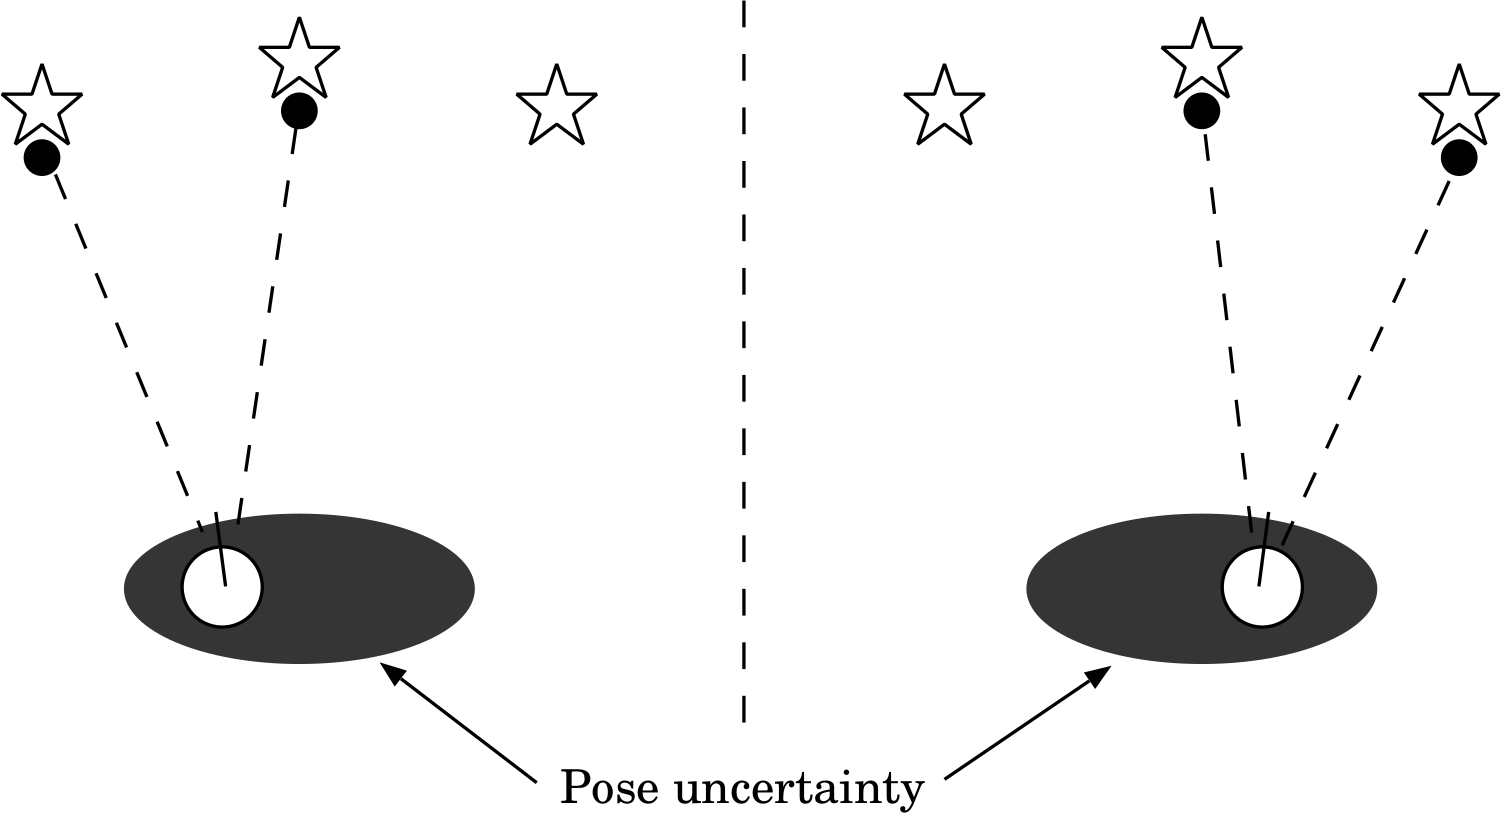
\includegraphics[width=0.5\linewidth]{fast_slam_data_association_problem}
	\captionwithcite{Zuordnung der Landmarken zu den Wahrnehmungen pro Pfadhypothese.}{\cite{thrun2005probabilistic}}
	\label{fig:fast_slam_data_association_problemn}
\end{figure}

Der \textit{FastSLAM} Algorithmus bildet die Grundlage für die beiden \gls{roslam} Verfahren die zum einen in den Abschnitten \autoref{sec:blanco2008pure} und \autoref{sec:blanco2008efficient} vorgestellt werden und zum anderen im der Evaluation ausgewertet.


%%%%%%%%%%%%%%%%%%%%%%%%%%%%%%%%%%%%%%%%%%%%%%%%%%%%%%%%%%%%%%%%%%%%%%%%%%%%%%%%
%
% - https://www.mrpt.org/tutorials/slam-algorithms/rangeonly_slam/
%
%%%%%%%%%%
%\subsection{RO-SLAM [todo]}


%%%%%%%%%%%%%%%%%%%%%%%%%%%%%%%%%%%%%%%%%%%%%%%%%%%%%%%%%%%%%%%%%%%%%%%%%%%%%%%%
%
%	- \url{https://www.heise.de/developer/artikel/Einfuehrung-in-das-Robot-Operating-System-3273655.html?seite=all}
%	- Node = Knoten
%	- Topic = Datenbus
%	- Service = Dienst
%	- Message = Nachricht
%	- Launch-Files = Startdateien
%
%%%%%%%%%%
\section{Robot Operating System}

Bei dem \Gls{ros} handelt es sich nicht im eigentlichen Sinne um ein Betriebssystem, sondern vielmehr um ein Framework das die Kommunikation zwischen verschiedenen Verarbeitungseinheiten regelt. Im Jahre 2007 begann die Entwicklung von \Gls{ros} an der Stanford University. Ab 2009 wurde dieses dann hauptsächlich an dem Robotik Institut Willow Garage weiterentwickelt. Durch die BSD Lizenz steht \Gls{ros} als Open-Source-Projekt sowohl der nicht-kommerziellen auch der kommerziellen Weiterentwicklung zur Verfügung. \cite{quigley2009ros}

Jedes \Gls{ros}-System muss über einen \Gls{ros}-Master verfügen. Dieser stellt den zentralen Punkt für die Registrierung von Knoten (engl. Nodes), Datenbusse (engl Topics) und Dienste (engl. Services) zur Verfügung.

Jeder Verarbeitungseinheit in \Gls{ros} wird durch einen Knoten repräsentiert. Ziel ist es möglichst kleine, wiederverwendbare und miteinander kombinierbare Einheiten zu bilden. Die Programmierung eines Knoten erfolgt dabei in den Programmiersprachen C++, Python oder Lisp.

Die Kommunikation zwischen den Knoten erfolgt dabei über ein \Gls{p2p}-Kanal auf der Basis von Nachrichten (engl. Messages). Bei einer Nachricht handelt es sich um eine Datenstruktur die primitive Datentypen, die Datentypstruktur anderer Nachrichten und Felder enthalten kann. Eine Nachricht wird dabei über das \textit{Publish-Subscribe} Muster in einem Datenbus veröffentlicht und kann von jedem Knoten empfangen werden der Nachrichten von diesem Datenbus abonniert hat. Der typische Anwendungsfall für dieses Verfahren ist die Bereitstellung von Sensordaten und Rückmeldungen über Statusänderungen.

Das zuvor vorgestellte \textit{Publish-Subscribe} Muster stellt eine asynchrone Kommunikation bereit. Mit Hilfe von Diensten ist auch ein synchroner Nachrichtenaustausch möglich. Hierfür wird eine Anfrage von dem \textit{Client} an den \textit{Server} gestellt, der seinerseits mit einem Ergebnis antwortet. Dieses Verfahren entspricht dem \textit{Request-Response} Muster. Die Erstellung einer inversen Transformation ist ein typischer Anwendungsfall hierfür.

Nach der Entwicklung neuer Algorithmen ist ein Vergleich mit den bereits bestehenden Algorithmen von großem Interesse. Mit dem Konzept der \textit{Bag}-Dateien können alle veröffentlichten Nachrichten aufgezeichnet werden und zu einem späteren Zeitpunkt wieder abgespielt werden.

Um die Wiederverwendbarkeit von Knoten, Nachrichten und Diensten zu fördern, wurde das Konzept der Pakete (engl. Packages) eingeführt. Ein Paket stellt die kleinste erstellbare Einheit dar und beinhaltet alle Teile eines Softwarepaketes wie z.B. Quellcode-, Konfigurationsdateien, Drittanbieter Bibliothek, Abhängigkeitslisten usw.

Eine Roboterplattform besteht aus vielen Sensoren und Aktuatoren die abgefragt und gesteuert werden müssen. Dementsprechend viele Knoten müssen gestartet werden. Diese Aufgabe erfüllen die Startdateien (engl. Launch-Files). Neben der Definition der Knoten die gestartet werden sollen, können Einzelne oder eine Gruppe von Knoten parametrisiert werden. Mittels der Verschachtelung von Startdateien ist eine Wiederverwendung von knotenspezifischen Startdateien möglich.

Zu den häufigsten Operationen der Verarbeitungseinheit einer Roboterplattform ist das Transformieren der Sensordaten aus dem Sensorkoordinatensystem in das Koordinatensystem des Robotermittelpunktes. In \Gls{ros} wird hier für ein Transformationsbaum (engl. TF-Tree) verwendet, der aus statischen und dynamischen Transformationen besteht. Statische Transformationen werden dort eingesetzt, wo sich die Pose zweier Koordinatensysteme zur Laufzeit nicht ändert, z.B. zwischen dem Robotermittelpunkt und einem fest montierten Sensor. Dynamische hingegen bei Koordinatensystemen die sich zur Laufzeit ändern, z.B. zwischen dem Robotermittelpunkt und den Inkrementalgebern der Antriebseinheit. Statische Transformationen können mittels einer \Gls{urdf}-Datei modelliert und allen Knoten bereitgestellt werden.

